\documentclass[12pt]{report}
\usepackage[print,nopanel]{pdfscreen}
\usepackage{lipsum}
%\usepackage{titletoc}
\usepackage{titlesec}
\titleformat{\chapter}[display]
{\normalfont\huge\bfseries}{\chaptertitlename~\thechapter}{20pt}{\Huge}
\titlespacing*{\chapter}{0pt}{50pt}{40pt}
\titlespacing*{name=\chapter,numberless}{0pt}{-30pt}{10pt}
\usepackage{lastpage}
\usepackage{macro/macro}
\usepackage{fancyhdr}
\usepackage{verbatim}
\usepackage[Glenn]{fncychap}
\usepackage{float}
\usepackage{booktabs}
\usepackage{array}
\usepackage{xcolor, colortbl}
\definecolor{Gray}{gray}{0.85}
\newcolumntype{K}[1]{>{\centering\arraybackslash}p{#1}}
\usepackage{placeins}
\let\Oldsection\section
\renewcommand{\section}{\FloatBarrier\Oldsection}
\let\Oldsubsection\subsection
\renewcommand{\subsection}{\FloatBarrier\Oldsubsection}
\let\Oldsubsubsection\subsubsection
\renewcommand{\subsubsection}{\FloatBarrier\Oldsubsubsection}
\lhead{\tiny\bfseries Linux Device Driver for BlueNRG}
\usepackage[left=2.5cm, right=1.5cm, top=2.5cm, bottom=1.5cm]{geometry}
\pagestyle{fancy}
\margins{2.5cm}{1.5cm}{1.5cm}{1.5cm}
\linespread{1.25}
\setlength\parindent{0pt}
\setcounter{tocdepth}{4}
\setcounter{secnumdepth}{5}

\begin{screen}
	\renewcommand{\encodingdefault}{T1}
	\usepackage{setspace}
	\linespread{1.5}
	\renewcommand{\rmdefault}{ptm}
\end{screen}
\screensize{8cm}{9cm}
\overlay{overlay8.pdf}
\usepackage{graphicx}
%\usepackage[compact]{titlesec}
%\titleformat{\chapter}[display]
%{\normalfont\huge\bfseries}{\chaptertitlename\\thechapter}{20pt}{\Huge}
%\titlespacing*{\chapter}{0pt}{0pt}{40pt}

\begin{document}
	\newcommand{\centertext}[1]{\begin{center}\textbf{#1}\end{center}}
\newcommand{\student}{\vskip 2.5cm}
\newcommand{\supervisor}{\vskip 2.5cm}
\newcommand{\stamp}{\vskip 2.5cm}
\newcommand{\HRule}{\rule{\linewidth}{0.5mm}}
\newcommand{\projecttitle}{\Huge \bf{Linux Device Driver \\for \\BlueNRG}\vskip 0.1in}
\newcommand{\tab}[1]{\hspace{.4\textwidth}\rlap{#1}}
\newcommand{\itab}[1]{\hspace{.05\textwidth}\rlap{#1}}
\newcommand{\logo}[1]{\includegraphics[scale=0.16]{#1}}
\newcommand{\submitted}{
	\vskip 0.1in
	\textnormal {Submitted for partial fulfilment of the Degree\\ of \\
		Bachelor of Technology\\
		(Computer Sceince and Engineering)\\}
	\vskip 1.0cm
	\logo{images/gne.png}
	\vskip 1.5cm

	\begin{minipage}{0.4\textwidth}
		\begin{flushleft} \large 
			{Submitted By:}\\
			\textnormal {Govind Sharma\\1311053\\135026}
		\end{flushleft}
	\end{minipage}
	\begin{minipage}{0.4\textwidth}
		\begin{flushright}\large 
			{Submitted To:}\\
			\textnormal {Sukhjit Singh Sehra\\ Training Coordinator\\ CSE Department\\}
		\end{flushright}
	\end{minipage}\\[2cm]
	\HRule\\[0.4cm]

	\textnormal{Department of Computer Science \& Engineering\\
	Guru Nanak Dev Engineering College\\
	Ludhiana 141006}
}

\newcommand{\pagetitle}{\begin{center}
\projecttitle
\Large\textbf{}\\
\submitted
\vskip 1cm
\end{center}}

%\newcommand{\openoffice}{\textbf}{OpenPffice}
\newcommand{\frontmatter}[1]{\begin{Large} \textbf{#1} \end{Large}}
\newcommand{\ppttitle}{\begin{center}
\end{center}}

	\begin{screen}
		\ppttitle
	\end{screen}
	\footskip 0.7cm
	\thispagestyle{empty}

	\pagetitle
	\newpage

	\pagenumbering{Roman}
	\cfoot{\thepage}

	\begin{Large}
	\centertext{Abstract}
\end{Large}

\vskip 0.1in
\noindent Bluetooth is a wireless technology standard for exchanging data over short distances. While exchanging data is the most accurate and popular use case of Bluetooth, the technology has transcended this simple initial purpose. Bluetooth is managed by the Bluetooth Special Interest Group (SIG), which has more than 25,000 member companies in the areas of telecommunication, computing, networking and consumer electronics. Bluetooth technology has found itself to be a perfect fit for many and many short distance communication problems, and has also re invented and improved itself over the years in order to keep up with the market trends. One such monumental change or addition to Bluetooth that is going to feature heavily in this report is Bluetooth Low Energy, a smarter and edgier version of Bluetooth.\\

\noindent Linux, a Unix-like and mostly POSIX-compliant, open souce OS kernel is also the most used kernel in operating systems varying from PCs, mobiles, SoCs, etc.\\

\noindent This project report documents in detail the integration of BlueNRG, A Bluetooth network processor by STMicroelectronics with the Linux kernel. A detailed account is presented of the study of Bluetooth Low Energy protocol stack, Linux device model, and all other things that contributed to the final product i.e. a Linux device driver for BlueNRG.

	\newpage

	\begin{Large}
\centertext{Acknowledgement}
\end{Large}
%\vskip 0.5cm
\noindent I, student of Guru Nanak Dev Engineering College, Ludhiana, have taken efforts in this project. However, it would not have been possible without the kind support and help of many individuals and organizations. I would like to extend my sincere thanks to all of them.\\

\noindent The author is highly grateful to Dr. M.S. Saini Director, Guru Nanak Dev Engineering College, Ludhiana for providing him with the opportunity to carry out his Six Months Internship at STMicroelectronics, Greator Noida.\\

\noindent The constant guidance and encouragement received from Dr. K.S. Mann, Dean T\&P, GNDEC Ludhiana, has been of great help in carrying out the training program and is duly acknowledged.\\

\noindent The author would like to whole heartedly thank Mrs. Shikha Singh and Mr. Raunaquq Quiserr for their constant guidance and direction. Without their help and motivation, it would not have been possible for this internship to go as smoothly and rewardingly as it did.\\

\noindent It is my absolute honor to place on record my best regards and deepest sense of gratitude to Mr. Manoj Kumar and all the mentors for their judicious and precious guidance and inspiration both of which were instrumental in growth as an engineer during my internship.\\

\noindent Finally, I would thank my fellow interns who have always uplifted my spirit and assisted in so many ways to my project.\\

\noindent Govind Sharma

	\newpage

	\tableofcontents
	\newpage

	\listoffigures
	\newpage

	\listoftables
	\newpage

	\pagenumbering{arabic}
	\cfoot{\thepage}

	\vskip -2cm
	\chapter{Introduction to Organiztion}
\begin{figure}[ht]
	\centering
	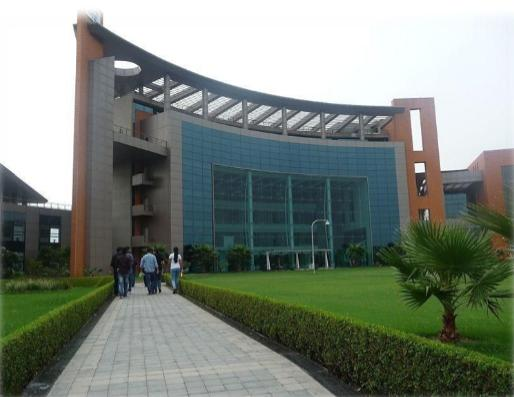
\includegraphics[width=3.5in, height=3in]{images/company.jpg}
	\caption{STMicroelectronics Pvt. Ltd., Greator Noida}
\end{figure}
\noindent STMicroelectronics is a world leader in providing the semiconductor solutions that make a positive contribution to people's lives, today and into the future.\\
\noindent Offering one of the industry's broadest product portfolios, ST serves customers across the spectrum of electronics applications with innovative semiconductor solutions for Smart Driving and the Internet of Things. %By getting more from technology to get more from life, ST stands for life.augmented.
\begin{itemize}
	\item Among the world's largest sermicondutor companies.
	\item A leading Integrated Device Manufacturer serving all electronics segments.
	\item A leading technology innovator (approximately 8,300 people working in R\&D, ~15,000 owned patents in ~9,000 patent families and 500 new patent filings).
	\item Delivering solutions that are key to Smart Driving and Internet of Things.
	\item Rich, balanced portfolio (ASICs, Application-Specific Standard Products and Multi-Segment Products).
	\item A pioneer and visionary leader in sustainibility.
	\item Corporate Headquarters: Geneva, Switzerland.
	\item President and CEO: Carlo Bozotti.
	\item 2015 revenue: \$6.90 billion.
	\item Approximately 43,200 employees.
	\item Over 75 sales \& marketing offices in 35 counteries.
	\item 11 main manufacturing sites.
	%\item Public ince 1994 - traded on New York Stock Exchange (NYSE: STM), Euronext Paris, and Borsa Italiana.
	\item Created as SGS-THOMPSON Microelectronics in June 1987, from merger of SGS Microelettronica (Italy) and Thomson Semiconducteurs (France).
	\item Renamed STMicroelectronics in May 1998.
\end{itemize}

	\newpage

	\chapter{Introduction to Project}
BlueNRG is a very low power Bluetooth low energy (BLE) single-mode network processor, compliant with Bluetooth specification v4.0. It has an embedded Bluetooth low energy protocol stack: GAP, GATT, SM, L2CAP, LL, RF-PHY. It can play both master and slave roles communicating with other devices or PCs using a proprietary Application Controller Interface (ACI) in addition to the standard Host Controller Interface (HCI) via SPI (Serial Peripheral Interface). 
\section{Overview}
In order to have two devices communicate with each other using Bluetooth, one needs to ensure that both devices are equipped with the enough hardware capability and apt software support. The fundamental component of a Bluetooth device is the Bluetooth radio and some necessary subset of the Bluetooth stack. BlueNRG is one such device. Like any other Bluetooth hardware device, BlueNRG can be used as an adapter to work with a host system that otherwise does not have the hardware to function Bluetooth. This use case makes BlueNRG a peripheral to a host i.e. A system on chip. \\
The host system must be able to communicate with BlueNRG in order set straight the relationships and interaction between various portions of the stack. These communications are of course handled by the Operating System. Furthermore for the OS to communicate with an external peripheral, device drivers are employed. And this is the whole idea of this project: creating a device driver for BlueNRG so that it can be used in conjunction with systems running on Linux based operating systems.\\
The device driver ensures that the peripheral is able to communicate with the host but the way this communication is to be conducted depends on what physical connection options are offered by the peripheral. In case of BlueNRG, the physical interface is SPI. Once the means of communication are fixed, there comes the question of deciding which part of the protocol is to reside on which side, the host or the peripheral. It will be seen in later chapters as to how the whole stack has been fragmented in this project.\\
Linux is written in C and so are the device drivers for Linux.

\section{Existing Systems}
Bluetooth has been a prominent technology in networking and has been the backbone of many user applications. As such it only makes sense that an operating system incorporates enough attention to Bluetooth as a technology. And this is exactly the case with Linux. It was realized early on that Bluetooth is going to be a major player and hence efforts were made to have it be an integral part of Linux. The software side of Bluetooth is official Bluetooth protocol stack for Linux which will be looked at in later sections of this report. The other major thing that then remains is the hardware: the Bluetooth adapter. In the modern computers mostly the Bluetooth adapter is inbuilt in the computer hardware itself but even if a Bluetooth adapter is not inbuilt into the system, there are a plethora of very inexpensive Bluetooth adapters in the market that can be used as plug and play peripheral to get Bluetooth working. This is of course possible because Linux, the OS has a stack support for Bluetooth, so once a hardware is detected then all that remains is to bridge this stack to the device using some standard protocol. All of this is taken care by the device driver for that particular device. It is simple, in order for a device to be supported, there has to be a device driver for it, and in this section I describe some of the widely used Bluetooth adapters that are supported by Linux at the time this writing:
\subsection{BlueFritz USB Bluetooth adapter}
The Bluetooth-Stick BlueFRITZ! USB allows you cordless connects to various Bluetooth devices. These can be, for example, access points for DSL or ISDN. It is very apt to connect to printers, mobile phones and PDAs. This allows better mobility, high speed, faster connection set-up and optimal line quality and maximum operational safety.
\begin{figure}[ht]
	\centering
	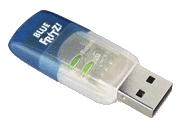
\includegraphics[scale=0.5]{images/bluefritz_usb.png}
	\caption{BlueFritz USB Bluetooth Adapter}
\end{figure}
\subsection{Qualcomm Atheros chips}
Qualcomm Atheros is a developer of  semiconductors  for  network  communications, particularly wireless chipsets. Qualcomm Atheros offers Bluetooth chips for a variety of platforms. The company also offers integrated combo WLAN and Bluetooth chips. In July 2008, Atheros released an open-source Linux driver for their 802.11n devices which includes its Bluetooth chipset as well. 
\begin{figure}[ht]
	\centering
	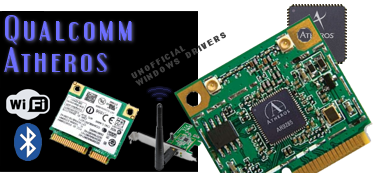
\includegraphics[width=3.5in, height=3in]{images/qualcomm_atheros.png}
	\caption{Qualcomm Atheros chips}
\end{figure}
Qualcomm Atheros’ Bluetooth solution is the AR3001 family of chipsets. The Qualcomm AR3001 is a highly integrated, all-CMOS, single-chip Bluetooth 2.1 and 3.0 + HS solution for mobile handset and portable electronics applications. The compact size and low power consumption of this AR3001 design make it an ideal vehicle for adding Bluetooth to hand-held and other battery-powered consumer electronic devices. The AR3001 supports the standard UART HCI interface and is therefore compatible with any upper layer Bluetooth stack. It is also designed to require less than 12 passive components, thus providing the lowest system BOM cost for mobile phone or portable consumer electronics applications. The AR3001 supports advanced architecture and protocol techniques to save power during sleep, stand-by and active states. The AR3001 family supports 2-, 3- and 4-wire Bluetooth coexistence protocols with advanced algorithms for predicting channel usage by the co-located WLAN transceiver in the same system. It supports all Bluez profiles. 
\subsection{Intel Bluetooth Devices}
Intel is a leading supplier of Bluetooth solutions, offering a product portfolio from mobile phones to automotive, industrial, and medical applications. Linux has drivers for Bluetooth devices offered by Intel.\\
They offer single-chip semiconductor solutions as well as system modules and integrated IP-block solutions to enable increased flexibility and optimization.\\
The Intel BlueMoon architecture is now in its sixth generation and offers a well-proven functionality and performance. Intel BlueMoon products offer superior RF performance along with innovative software solutions for high quality operation. The Intel BlueMoon product family has been designed for voice quality and high-performance data transmissions with reduced requirements on the host processor.\\
Their single solutions are small and cost-effective, targeting mobile phones, automotive, industrial, and medical applications. Intel’s module solutions are Bluetooth qualified, offering an accelerated time to market and lower initial investments.\\
Intel is one of the seven promoters of the Bluetooth SIG and has participated in Bluetooth standardization since the start of Bluetooth.
\begin{figure}[ht]
	\centering
	
\includegraphics[width=3.5in, height=3in]{images/intel_bluetooth.png}
	\caption{Intel Bluetooth Devices}
\end{figure}
\subsection{Broadcom Blutonium}
The Blutonium BCM2045 is the primary single-chip solution for Bluetooth applications, designed from the ground up to promote and enable the adoption of Bluetooth in phones, computers, peripherals and other devices. The chip exhibits stellar features like low power consumption, board space, radio performance and low cost. The chip supports the new Bluetooth Extended Data Rate (EDR), providing raw bandwidth of 3 Megabits per second for wireless applications. In addition, Broadcom’s inConcert interference avoidance technology reduces possible disruption from nearby Wi-Fi products, which operate in the same 2.4 GHz radio frequency as Bluetooth.
\begin{figure}[ht]
	\centering
	
\includegraphics[width=3.5in, height=3in]{images/broadcom_blutonium.png}
	\caption{Broadcom Blutonium}
\end{figure}
\subsection{Marvell Bluetooth}
88W8689 constitutes Marvell’s family of Bluetooth solutions among other solutions as well. With the addition of 88W8689, Marvell now provides a comprehensive set of Bluetooth 2.0-enabled products that target high-volume consumer markets. The highly integrated chip is optimized for both voice and audio transmissions, enabling an array of ultra-mobile, low-power consumer devices. \\
There are other solutions by Marvell for Bluetooth as well and they work well with Linux as the driver is there for them.
\begin{figure}[ht]
	\centering
	
\includegraphics[width=3.5in, height=3in]{images/marvell_bluetooth.png}
	\caption{Marvell Bluetooth}
\end{figure}
\subsection{3Com Bluetooth PCMCIA Card}
The 3Com Wireless Bluetooth PC Card is a Bluetooth version 1.1 device, but 3Com refers it as Version 2.0. Two applications are included: 3Com Bluetooth Mobile Connection Manager, for mobile communications configuration outside the Bluetooth network, and 3Com Bluetooth Connection Manager. The 3Com PC Card adapter provides a well-designed and easy-to-use solution with the antenna retracted, the device sits flush with the edge of your notebook’s Type II PC Card slot, making it easy to transport. You can even leave the PC Card in your notebook permanently so that you’re always prepared to connect with other Bluetooth-enabled devices. While leaving the 3Com card in your computer will cause minimal battery drain, you can always disable the adapter by ejecting it.\\
The PC Card is easy to install and has support in Linux kernel as well.
\begin{figure}[ht]
	\centering
	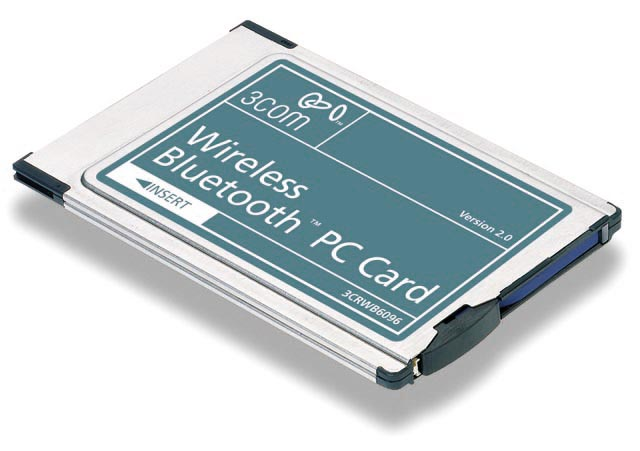
\includegraphics[width=3.5in, height=3in]{images/3com_bluetooth.png}
	\caption{3Com Bluetooth PCMCIA Card}
\end{figure}
\subsection{Texas Instrument Dual-mode Bluetooth CC2564 Module}
The CC2564MODAEM evaluation board contains the Bluetooth BR/EDR/LE HCI solution. Based on TI's CC2564B dual-mode Bluetooth single-chip device, the bCC2564MODA is intended for evaluation and design purposes, reducing design effort and enabling fast time to market. This module has the following set of features:
\begin{itemize}
	\item CC2564MODN device (MOE package)
	\item Bluetooth Specification v4.1
	\item Dual Mode - Bluetooth \& Bluetooth low energy
	\item FCC, IC, CE certified
	\item Class 1.5 Transmit Power (+10dBm)
	\item High sensitivity (-93 dBm typ.)
	\item UART Interface - Control and Data
	\item PCM/I2S Interface - Voice and Audio
	\item 4 Layer PCB design
	\item 1.8 LDO (LP2985-18)
	\item 3 Voltage level translators (SN74AVC4T774)
	\item Chip antenna (LTA-5320-2G4S3-A1) and RF connector (U.FL-R-SMT-1)
	\item EM connectors that plug directly into the TI hardware development kits:
	\begin{itemize}
		\item MSP-EXP430F5529
		\item MSP-EXP430F5438
		\item DK-TM4C123G
		\item DK-TM4C129X
	\end{itemize}
	\item COM connector
	\item Certified and royalty-free TI Bluetooth Stack
\end{itemize}

\section{Requirement Analysis}
There are many Bluetooth adapters out there that have well documented and tested support in Linux based operating systems. Linux being an open source kernel is always inviting people to look into its internal working and stack flow in order to contribute in it.\\
STMicroelectronics excels at grabbing newer opportunities and always be ready with solutions that are on par or even transcends other solutions in the market in a wide range of technologies. The Bluetooth technology is no different. ST has its fair share of Bluetooth modules. Along with the Bluetooth Smart technology, ST has also offered modules that serve complaint to that specification. But thing to be considered here is that even though ST has a wide range of Bluetooth solutions, none has Linux support. \\
So the major requirement of this project was to take a Bluetooth module by ST and add its support to Linux. And again Linux being open source makes the job much simpler. The module that was considered is the BlueNRG module which is Bluetooth 4.0 complaint. This means that it has the much coveted Bluetooth Smart (Low Energy) features. So the whole requirement of this project can be summed up as adding support (writing a device driver) in Linux (because it is open source and one of the most popular OS kernels in the world) for the BTLE module offered by STMicroelectronic i.e. BlueNRG.\\
In order to fulfill the above stated requirement it is essential to look into both sides of the coin: Linux driver development and how is the Bluetooth stack being represented there; and then BlueNRG and what portion of the stack is on it and how much of it is needed in order to work with Linux.\\
The official Bluetooth protocol stack for Linux is Bluez. Bluez is designed in such a way that it offers the HCI interface to any adapter that wish to communicate through it. So for a Bluetooth adapter to be connected to a Linux host, and wanting to utilize the Bluez protocol stack, it needs to extend the HCI interface. And since HCI is also part of the Bluetooth standard, it is not very hard have all Bluetooth devices follow the same protocol. If communication between the host and the controller is to be had using the Bluez protocol stack then it has to happen through the Host Controller Interface as defined in the Bluetooth specification document.\\
Now comes the question of whether BlueNRG is capable of HCI communication, to which the answer is a definite yes. As it will be seen later in this report, BlueNRG is designed to communicate using the Application Controller Interface (ACI), which is a proprietary protocol. But the good news is that ACI is almost a super set of the standard HCI protocol. Since ACI is proprietary and Linux Bluetooth stack offers communication to all devices through only the HCI protocol, it becomes essential to use only the HCI subset available for BlueNRG. Another important point to consider is that how the connection is to be made between the Host (running on Linux) and BlueNRG controller. BlueNRG is based on Serial Peripheral Interface, so that is exactly what is required to be used for the connections. 

\section{Feasibility Study}
As stated in the requirement analysis section, there are two things that are needed to considered here:
\subsection{ Does BlueNRG support what Bluez offers?}
The answer is yes. Bluez interfaces with any device or adapter using the Host Controller Interface which is essentially a protocol standard defined in the Bluetooth specification itself as a means to communicate between the host and the controller. Since BlueNRG is responsive to HCI commands, all seems to be set here. The communication between the host and the controller are to be had through HCI commands (send from the host) and HCI events (generated by the controller in response to the commands send by the host). According to the ACI programing manual, HCI is indeed the subset of ACI. So BlueNRG should be able to respond to HCI commands offered by Bluez of Linux.
\subsection{Does Linux supports what BlueNRG uses to communicate through?}
BlueNRG is based on SPI. Any form of communication between the host and BlueNRG is to be had through the Serial Peripheral Interface. While there isn’t a SPI based Bluetooth driver in Linux at the time of this writing, but there certainly is a rich SPI support in Linux. There are many network drivers that allow the communication between the host and the controller through SPI. So following the same footsteps it should be possible to send commands (HCI) from the host to the controller using SPI.\\
Considering the above things, it seems feasible to write a driver for BlueNRG in Linux. The driver shall essentially act as a bridge between Bluez protocol stack residing partly in the user space and partly in the kernel space of Linux and BlueNRG. Every Bluetooth action that is needed to be performed will be in the form of an HCI command, which is what the driver should expect from Bluez and interface it through SPI to BlueNRG.

\section{Obejectives of the Project}
\begin{itemize}
	\item To setup a Bluetooth driver interface for SPI.
	\item To filter HCI commands to the ones that are supported by BlueNRG.
	\item To interface HCI commands from Bluez stack to BlueNRG.
	\item To map Bluez commands to the BlueNRG functionalities.
\end{itemize}


	\newpage

	\chapter{Product Design}
\section{Product Functions}
When complete the device driver should be able to fully facilitate a communication between the host and the controller. This means that all the features supported by BlueNRG must function depending on how the user is willing to use them through the host. To learn more about the functionality offered by BlueNRG, one needs to go through BLE, what is is and what it has to offer. The subsequent sections of the report present a detailed case of the same.
\subsection{Bluetooth Low Energy}
Bluetooth low energy (\textbf{BLE}, marketed as \textbf{Bluetooth Smart}) is a wireless personal area network technology designed and marketed by the \textbf{Bluetooth Special Interest Group aimed} at novel applications in the healthcare, fitness, beacons, security, and home entertainment industries. \\
It is part of the Bluetooth \textbf{4.0 specification}. It aims at being a low energy, low cost, low bandwidth, low power and low complexity extensible framework for exchanging data pertaining to various applications fields. 
\subsubsection{Device Configuration}
\begin{itemize}
	\item \textbf{Single mode Devices} (Bluetooth smart): These devices are compatible to BLE only. Examples are typically small devices like Heart monitors, sensors, other low-power consuming application hardware.
	\item \textbf{Dual mode Device} (Bluetooth smart ready): These device are compatible to both BLE and traditional BR/EDR. Example of this kind of devices are PCs, Tablets and smartphones i.e. devices with larger battery or power consumption.
\end{itemize}
\begin{figure}[ht]
	\centering
	
\includegraphics[scale=0.5]{images/device_configuration.png}
	\caption{BLE Device Configuration}
\end{figure}
\subsubsection{Limitations}
Bluetooth Low Energy has been designed with some specific fundamentals that happen to serve in a lot of application fields. But this means that it is not apt other kind of applications. Most of its limitations are due to the following two fundamental fact
\begin{enumerate}
	\item The maximum theoretical throughput is \textbf{1Mbps} which is reduces by several factors to only \textbf{5-10KBps} in most cases
	\item The operating range is generally \textbf{2-5 meters}. This can be extended to \textbf{30 meters} or so but that will of course demand higher strain on the battery life of the devices. This is the defining thing about the BLE technology that the devices are mostly passive in nature and hence it becomes very important for them to have large battery life. In some cases it is seen that the device’s battery can actually outlast other hardware in the device itself
\end{enumerate}
\subsubsection{Bluetooth Low Energy Network Topologies}
Network topology defines the way in which different devices (under different roles) interact with one another to exchange data through BLE. These topologies are defined within the specification and are maintained under the guidelines established by Generic Access Profile (GAP).\\
Following three topologies are found in BLE:
\begin{enumerate}
	\item Broadcasting and Observing
	\item Connection oriented
	\item Mixed topology
\end{enumerate}
Let’s take a look at them individually.
\paragraph{Broadcasting}
A device (broadcaster) sends out advertising packets (after fixed intervals) to any device that is willing to scan this packet and extract data from it. The observing device also scans for any advertising packets in its range after a fixed interval. When these two intervals (advertising and scanning) overlap, then the devices are able to exchange data among themselves.\\
Data broadcasting by a device can be picked up any observer. Observer can choose to acknowledge this reception or not.\\
Advertising packets contains data up to \textbf{31 bytes}. This can be extended by another packet if requested by any observer using the \textbf{scan request packet}.
\begin{figure}[ht]
	\centering
	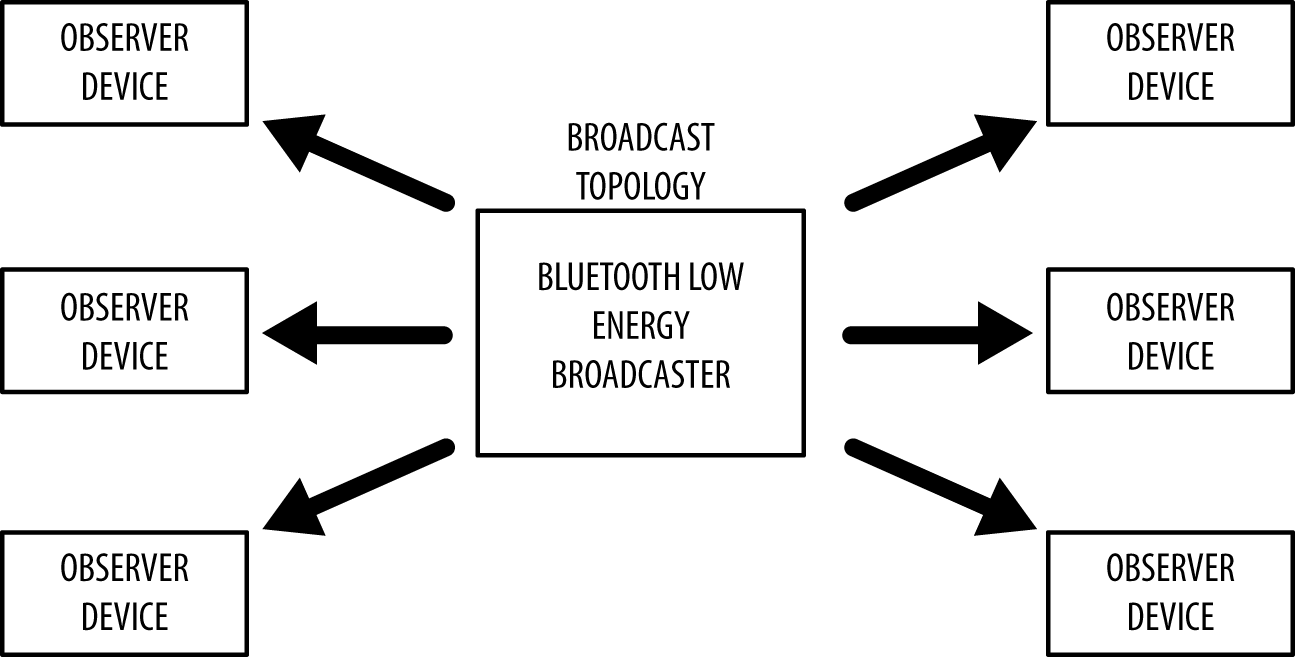
\includegraphics[width=3.5in, height=3in]{images/broadcast_topology.png}
	\caption{Broadcasting and Observing Topology}
\end{figure}
\paragraph{Connections}
A connection is a permanent, periodical data exchange of packets between two devices. It is therefore inherently private (the data is sent to and received by only the two peers involved in a connection, and no other device unless it is indiscriminately sniffing).\\
This topology is useful when one wants to communicate in both directions and the data to be communicated cannot be accommodated in two advertising packets.\\
Connections involve two separate roles: \textbf{Master} (scans for any device advertising to be in a connection) and \textbf{Slave} (advertises at intervals to be a part of an exclusive connection and accepts a connection request from a master to establish the connection).
\begin{figure}[ht]
	\centering
	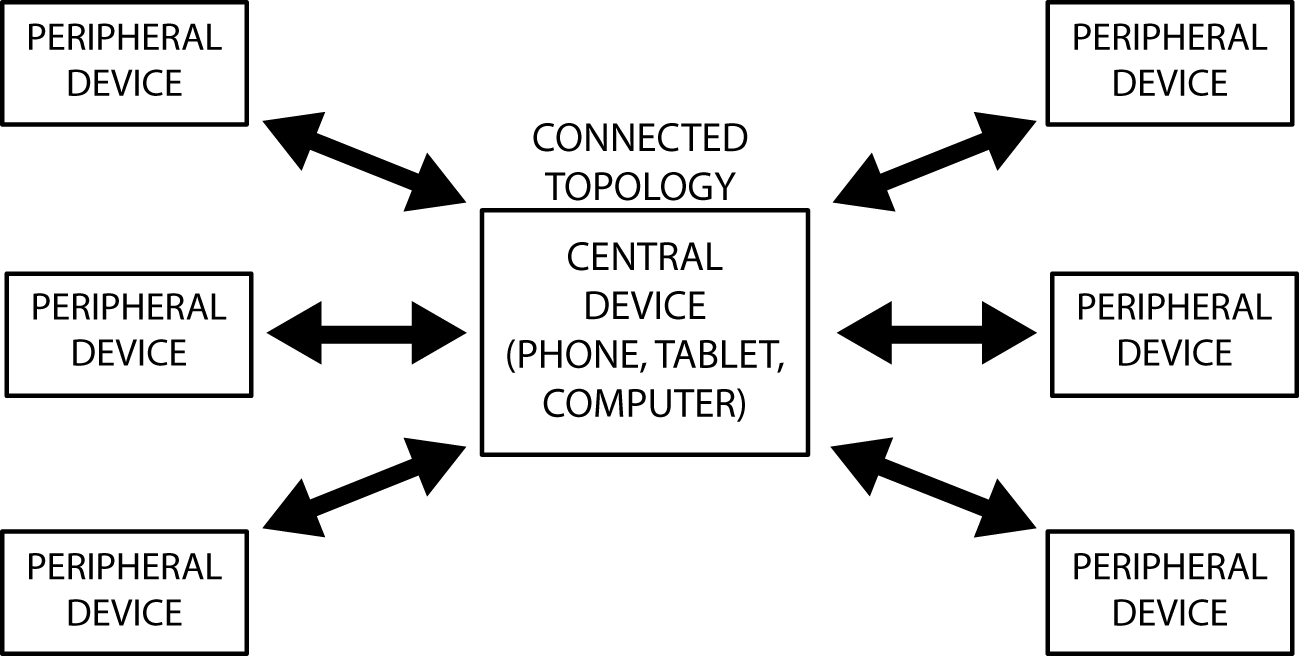
\includegraphics[width=3.5in, height=3in]{images/connected_topology.png}
	\caption{Connection Topology}
\end{figure}
\paragraph{Mixed Topology}
The previous two topologies can be mixed freely in a wider BLE network, as shown in the figure below. A BR/EDR/LE capable device can bridge together BLE and BR/EDR connections, and the number of combinations and participants on the network is constrained only by the limitations of the radios and protocol stacks of each device taking part in it.
\begin{figure}[ht]
	\centering
	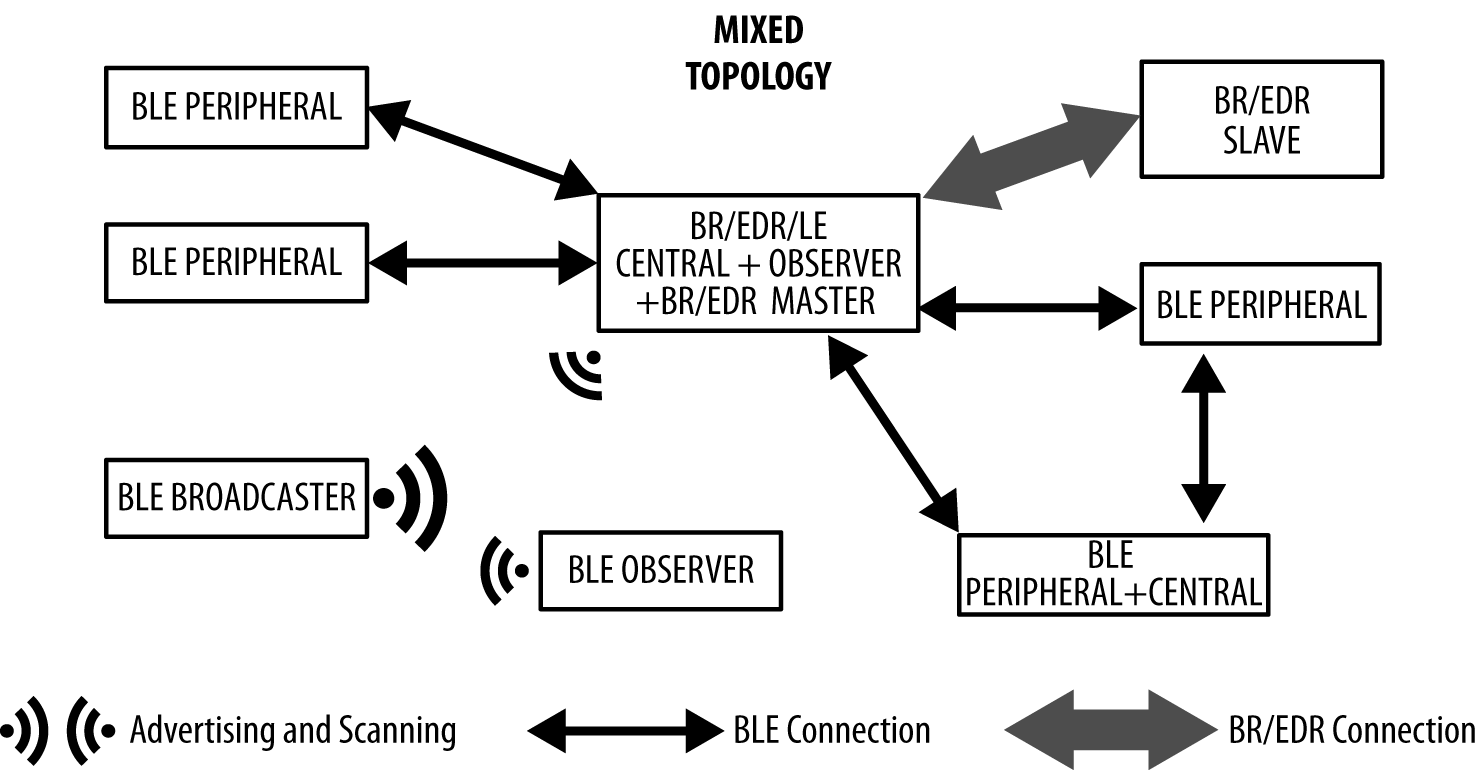
\includegraphics[width=3.5in, height=3in]{images/mixed_topology.png}
	\caption{Mixed Topology}
\end{figure}
\subsubsection{BLE Architecture}
The complete BLE protocol stack is divided into layers that work and communicate in succession to achieve the desired operation.\\
These layers are:
\begin{enumerate}
	\item \textbf{Application} (The upper layer containing most of the application logic, User interface, etc)
	\item \textbf{Host} (Contains all the upper layer protocols like GAP, GATT, L2CAP, etc.)
	\item \textbf{Controller} (Contains all the lower layer protocols from the Link Layer and the Physical Layer.)
\end{enumerate}
The host layer and the controller layer communicate with each other using the \textbf{Host Controller Interface} (HCI). This allows great flexibility in having the host and controller on different chips and having different manufactures.
\begin{figure}[ht]
	\centering
	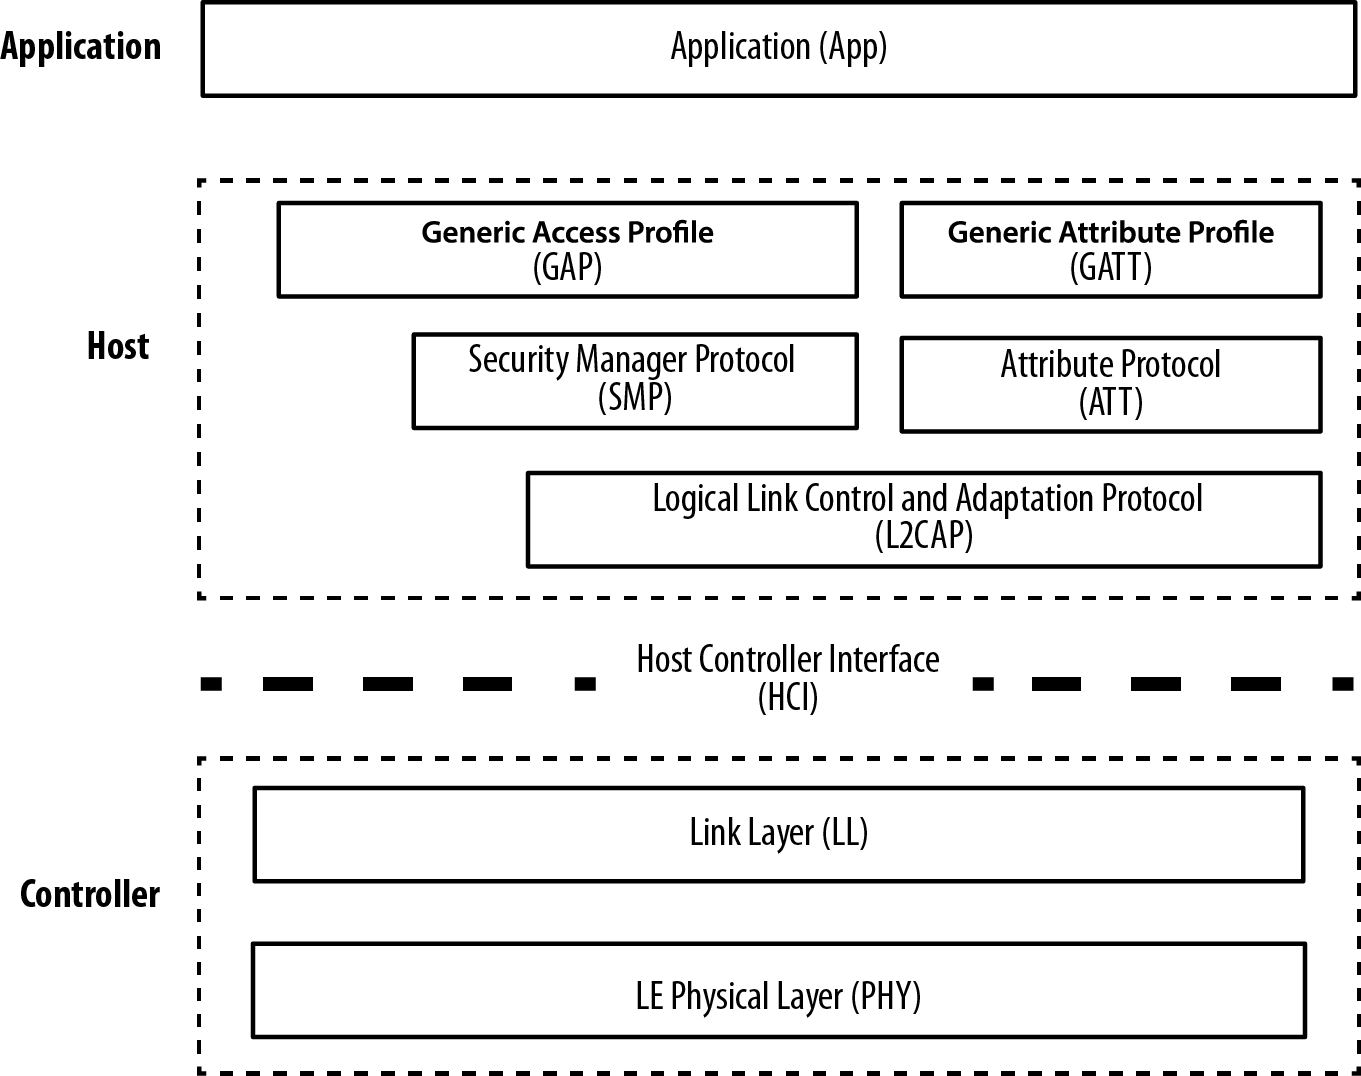
\includegraphics[scale=0.2]{images/ble_architecture.png}
	\caption{BLE Architecture}
\end{figure}
\subsubsection{Classification of devices based on Chip Count}
Like devices can be classified on the basis of different compatibility modes, they can also be classified on the basis of the chip configuration of the various layers of BLE.
\begin{enumerate}
	\item \textbf{SoC (System on Chip)}: A single IC runs the application, the host, and the controller.
	\item \textbf{Dual IC over HCI}: One IC runs the application and the host and communicated using HCI with a second IC running the controller.
	\item \textbf{Dual IC with connectivity device}: One IC runs the application and communicates using a proprietary protocol with a second IC running both the host and the controller. BlueNRG uses this chip configuration.
\end{enumerate}
\begin{figure}[ht]
	\centering
	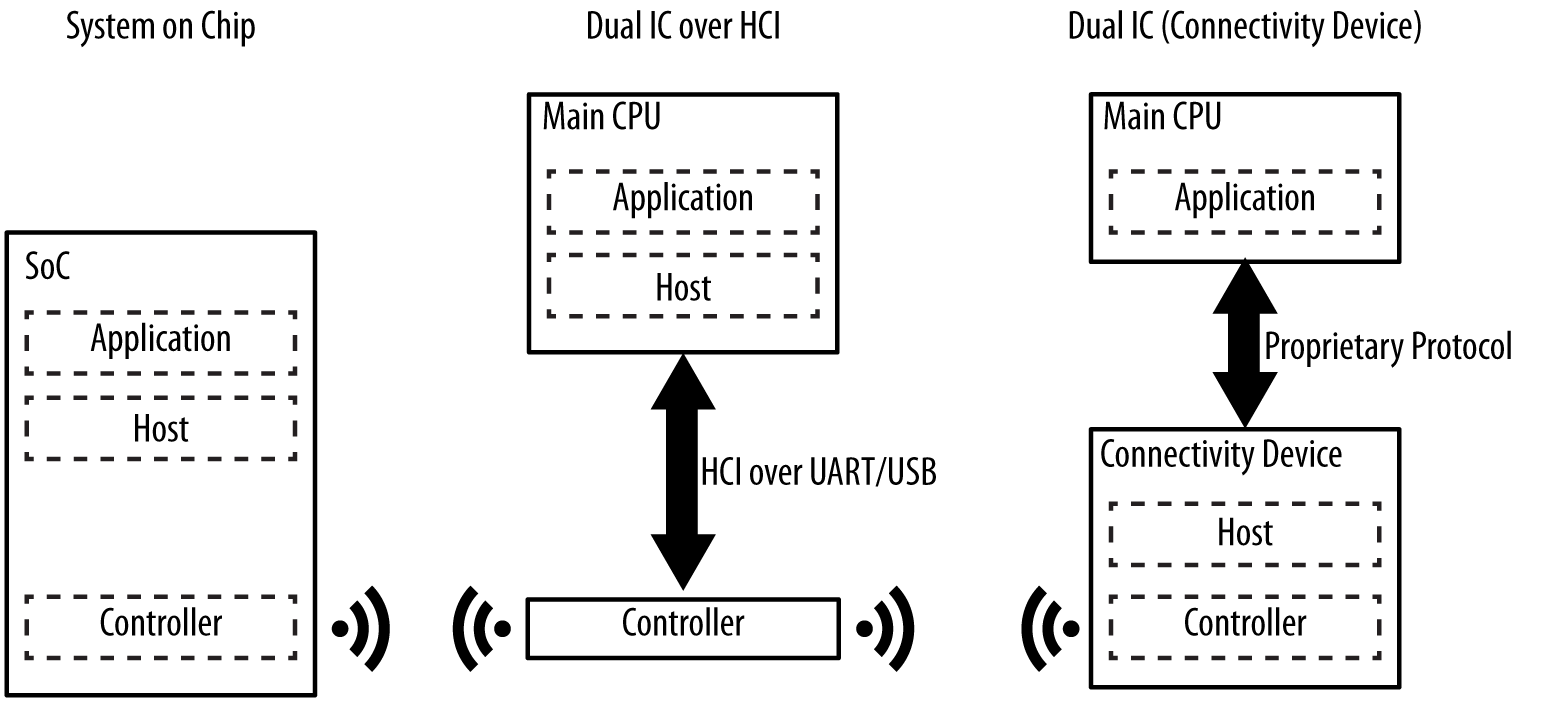
\includegraphics[scale=0.2]{images/chip_count.png}
	\caption{Classification based on chip count}
\end{figure}
\subsubsection{The Protocol Stack}
The whole BLE protocol stack is divided into layers. This makes it easier to study and apply the protocol because otherwise the protocol is not as plainly vertical as some other protocols are like the TCP/IP. The layers are:
\begin{enumerate}
	\item \textbf{The Controller Layer}
	\item \textbf{The Host Layer}
	\item \textbf{The Application Layer}
\end{enumerate}
\subsubsection{The Controller Layer}
This contains the lower layer of protocol like:
\paragraph{The Physical Layer}
This layer is responsible for the analog transmission and AC-DC conversions. Bluetooth utilized the 2.4 GHz ISM bandwidth with 40 2MHz channels. Out of these 40 channels, 37 are for data transfer that is to occur once the connection has been established between participating devices. The other 3 channels are for broadcasting, observing and advertising.\\
The specification uses the frequency hopping spread spectrum to prevent overlapping interference of channels. This hopping takes place simultaneously and is based on the following equation:\\
Channel = (CurrentChannel + Hop) mod 37\\
The modulus of 37 obviously is there to round of the channel number to stay between 0 and 36 i.e. the available data channels for connections. The value of hop is known only to the connected devices and this hence enables them to hop to the same channels at the same time and no one else will be able to interfere between them.
The Gaussian Frequency Shift Keying (\textbf{GFSK}) is used to encode the bit stream over the air.
\begin{figure}[ht]
	\centering
	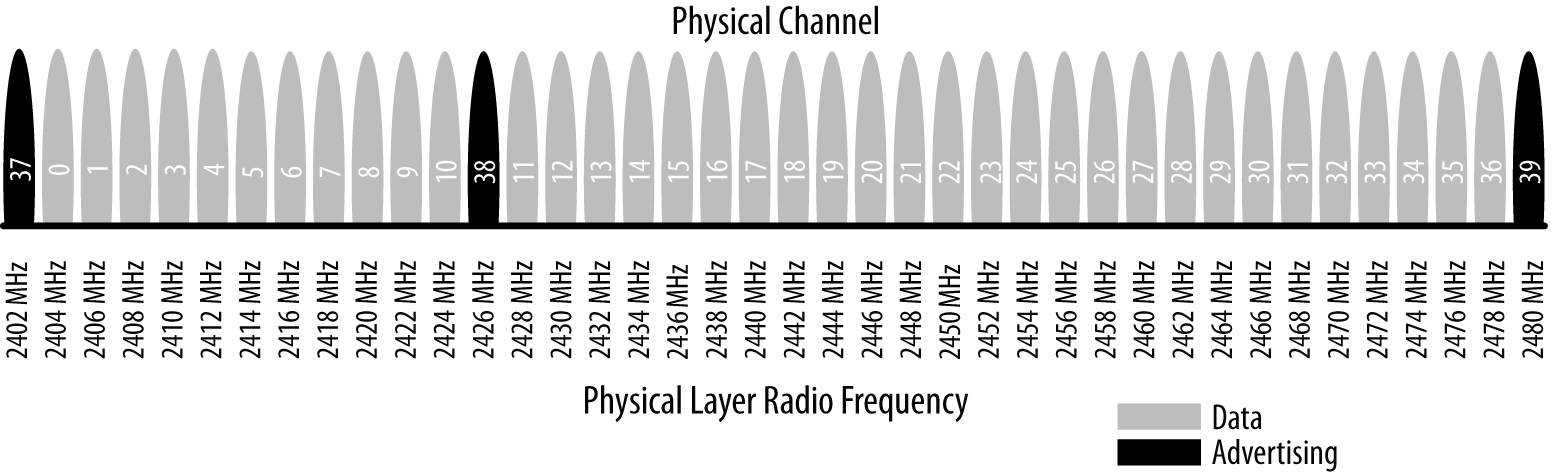
\includegraphics[scale=0.3]{images/physical_channel.png}
	\caption{The 40 physical channels}
\end{figure}
\paragraph{Link Layer}
The Link Layer is responsible for complying with all of the timing requirements defined by the specifications and managing device connections. It also performs CRC, Data whitening, Random number generations, AES encryption, etc.\\
The Link Layer defines the following roles:
\begin{enumerate}
	\item \textbf {Advertiser}: A device sending advertising packets.
	\item \textbf {Scanner}: A device scanning for advertising packets.
	\item \textbf {Master}: A device that initiates a connection and manages it later.
	\item \textbf {Slave}: A device that accepts a connection request and follows the master’s timing.
\end{enumerate}
These roles can be logically grouped into two pairs: advertiser and scanner (when not in an activie connection) and master and slave (when in connection).
\subparagraph{Link Layer Bluetooth Device Addresse}
This is the fundamental identifier of a Bluetooth device, similar to an Ethernet Media Access Control (MAC) address. It is \textbf{ 6 bytes} long. \\
There are two types of device addresses, and on or both can be set on a particular device:
\begin{enumerate}
	\item \textbf{Public Device Address}: This is factory-programmed device address. Registered with \textbf{IEEE} registration authority and never changes during the lifetime of the device.
	\item \textbf{Random Device Address}: This address can either be preprogrammed on the device or dynamically generate at runtime. It can be used to achieve privacy when in a connection.
\end{enumerate}
\subparagraph{Link Layer Advertising and Scanning}
The advertising packets are used to either broadcast data for applications or to discover slaves and to connect to them. The advertising of packets is done after certain intervals and if during this interval some device is scanning then that device will be able to receive the advertising packet.\\
The specification defines two basic types of \textbf{scanning procedures}:
\begin{enumerate}
	\item \textbf{Passive Scanning}: The scanner simply listens for advertising packets, and the advertiser is never aware of the fact that one or more packets were actually received by a scanner.
	\item \textbf{Active Scanning}: The scanner issues s Scan Request packet after receiving an advertising packet. The advertiser receives it and responds with a Scan Response packet. This additional packet doubles the effective payload that the advertiser is able to send to the scanner, but it is important to note that this does not provide a means for the scanner to send any user data at all to the advertiser.
\end{enumerate}
\begin{figure}[ht]
	\centering
	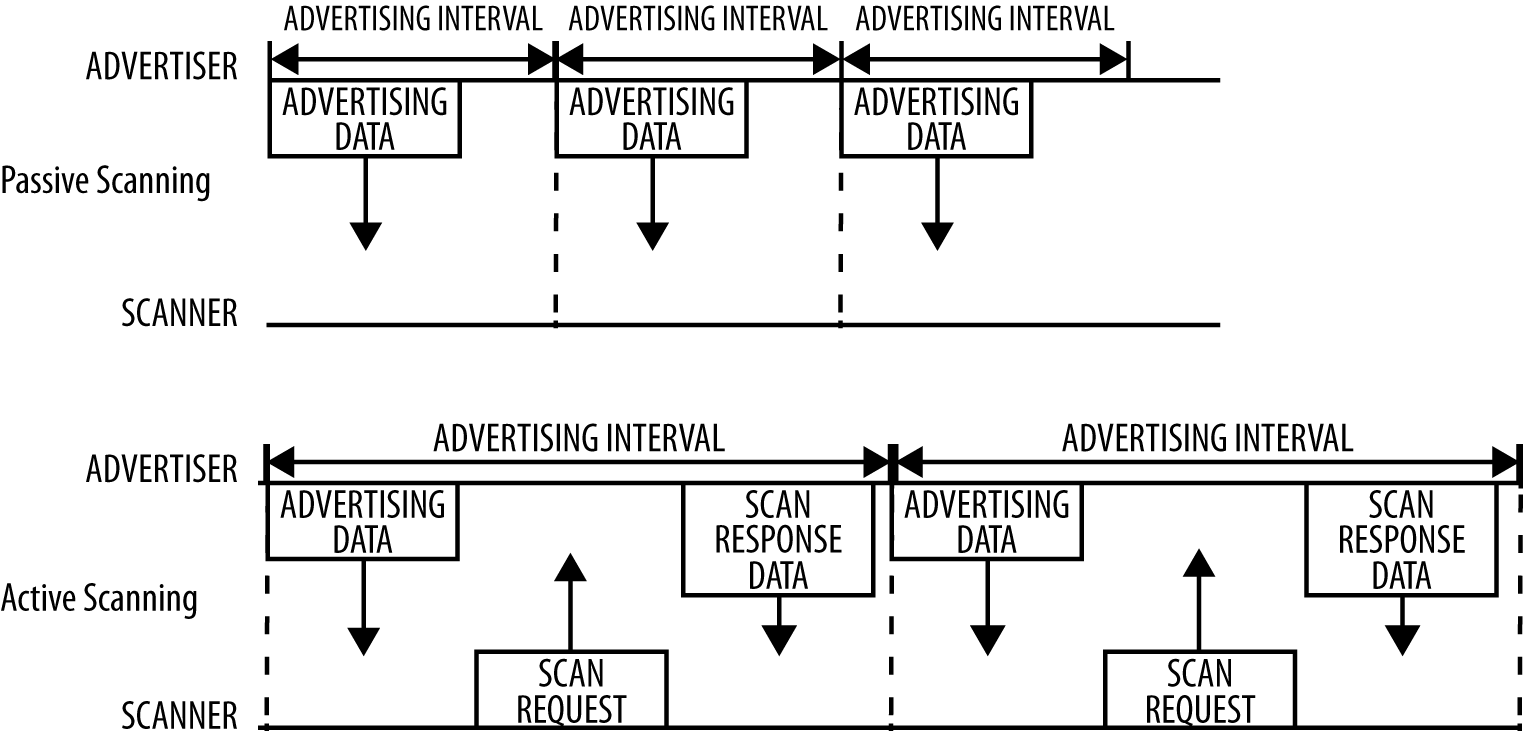
\includegraphics[scale=0.2]{images/advertising_scanning.png}
	\caption{Link Layer Advertising and Scanning}
\end{figure}
\subparagraph{Link Layer Advertising Packet types}
\begin{figure}[ht]
	\centering
	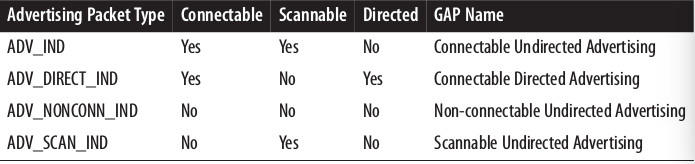
\includegraphics[scale=0.5]{images/advertising_packet_types.png}
	\caption{Link Layer Advertising Packet types}
\end{figure}
\subparagraph{Link Layer Connections}
To establish a connection, a master first starts scanning to look for advertisers that are currently accepting connection requests. A connection is simply a sequence of data exchanges between the slave and the master at predefined times. Shown in Figure, each exchange is called \textbf{connection event}.
\begin{figure}[ht]
	\centering
	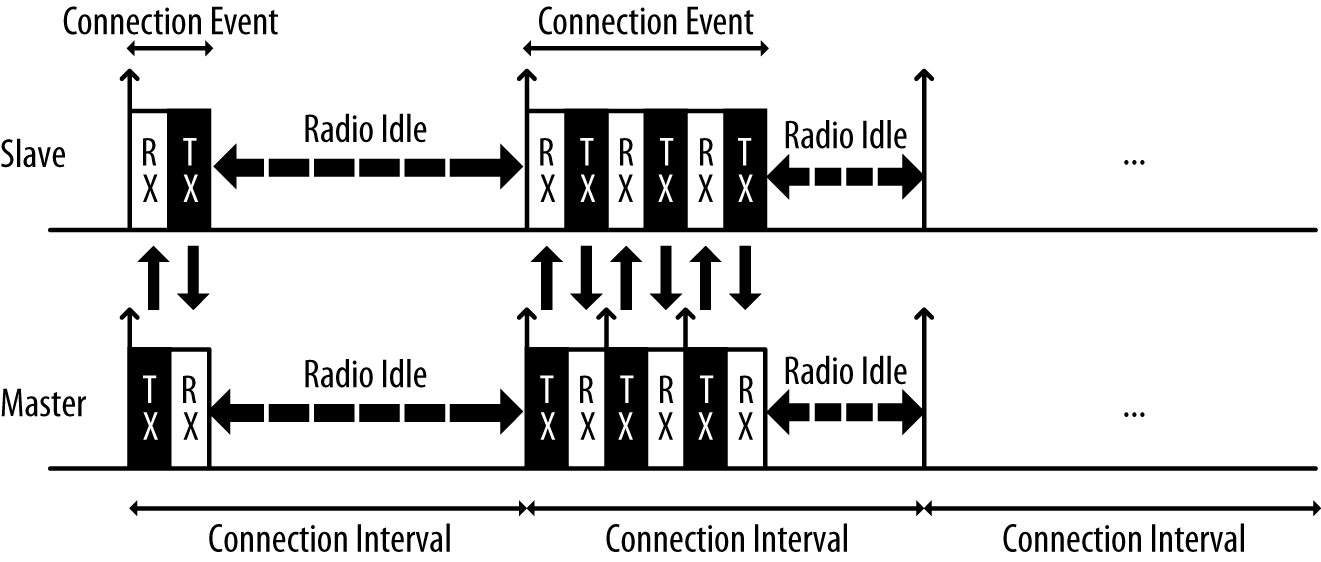
\includegraphics[scale=0.35]{images/connection_event.png}
	\caption{Link Layer connection event}
\end{figure}
\subparagraph{Link Layer connection parameters}
\begin{enumerate}
	\item \textbf{Slave latency}: The number of connection events that a slave can choose to skip without risking a disconnection.
	\item \textbf{Connection interval}: The time between the beginnings of two consecutive connection events. This value ranges from 7.5 ms (high throughput) to 4s (lowest possible throughput but also least power hungry).
	\item \textbf{Connection supervision timeout}: The maximum time between two received valid data packets before a connection is considered lost.
\end{enumerate}
\subsubsection{The Host Layer}
This layer contains many of the protocols and profiles of BLE stack that are essential to the functioning of the upper layers of BLE. Some of these are:
\begin{itemize}
	\item L2CAP
	\item SMP
	\item GAP
	\item ATT
	\item GATT
\end{itemize}
\paragraph{L2CAP}
\textbf{Logical Link Control and Adaptation Protocol} provides two main pieces of functionality:
\begin{enumerate}
	\item It serves as a \textbf{protocol multiplexer} that takes multiple protocols from the upper layers and encapsulated them into the standard BLE packet format (and vice versa).
	\item It also performs \textbf{fragmentation and recombination}, a process by which it takes large packets from the upper layers and breaks them up into chunks that fit into the 27-byte maximum payload size of the BLE packets on the transmit side. On the reception path, it receives multiple packets that have been fragmented and recombines them into a single large packet that will then be sent upstream to the appropriate entity in the upper layers of the host.
\end{enumerate}
\paragraph{ATT}
\textbf{The Attribute Protocol} (ATT) is a simple client/server stateless protocol based on attributes presented by a device. In BLE, each device is a client, a server, or both, irrespective of whether it is a master of slave. A client requests data from a server, and a server sends data to clients. Each server contains data organized in the form of attributes each of which is assigned a \textbf{16-but attribute handle}, a \textbf{universally unique identifier} (UUID), a \textbf{set of permissions}, and finally of course, a \textbf{value}. The attribute handle is simply an identifier used to access an attribute value. The UUID specifies the type and nature of the data contained in the value. \\
The client and server perform various operations under this protocol such as searching for attributes, reading the values of attributes, writing values to attributes, etc. All of these operations are allowed based on the attribute permissions.
\paragraph{SM}
\textbf{The Security Manager} (SM) is both a protocol and a series of security algorithms designed to provide the Bluetooth protocol stack with the ability to generate and exchange security keys, which then allow the peers to communicate securely over an encrypted link, to trust the identity of the remote device, and finally to hide the public Bluetooth Address if required to avoid malicious peers tracking a particular device.\\
The defined two roles, \textbf{Initiator} (always corresponds to the link layer master and therefor the GAP central) and \textbf{Responder} (link layer slave and hence the GAP peripheral).
\subparagraph{SM Security Procedures}
The Security Manager provides support for the following three procedures:
\begin{enumerate}
	\item \textbf{Pairing}: Exchanging of the temporary key generated by the devices. This is done using algorithms like \textit{Just works, Passkey display, and Out of Band.}
	\item \textbf{Bonding}: Saving the key shared during pairing for future connections.
	\item \textbf{Encryption re-establishment}: Using the key stored during bonding to re-establish the connection.
\end{enumerate}
\subparagraph{SM Security Mechanisms}
The SM specifies the following three types of security mechanisms that can be used to enforce various levels of security while in a connection or during the advertising procedure:
\begin{enumerate}
	\item \textbf{Encryption}: This mechanism consists of the full encryption of all packets transmitted over an established connection.
	\item \textbf{Privacy}: The privacy feature allows an advertiser to hide its public Bluetooth address by using temporary, randomly generated addresses that can be recognized by a scanner that is bonded with advertising device.
	\item \textbf{Signing}: With this mechanism, a device can send and unencrypted packet over an established connection that is digitally signed i.e. the source of which can be verified.
\end{enumerate}
\paragraph{GAP}
\textbf{The Generic Access Profile} (GAP) dictates how devices interact with each other at a lower level, outside of the actual protocol stack, GAP can be considered to define the BLE topmost control layer, given that it specifies how devices perform control procedures such as devices discovery, connection, security establishment, and other to ensure interoperability and to allow data exchange to take place between devices from different vendors.
\subparagraph{GAP Roles}
\begin{itemize}
	\item \textbf{Broadcaster}: Sends advertising packets for the purpose of broadcasting data.
	\item \textbf{Observer}: Scans for any broadcasted advertising packets in its range.
	\item \textbf{Central}: Scans for any advertising packet that is inviting a connection with a peripheral.
	\item \textbf{Peripheral}: Sends advertising packets for the purpose of connecting with a central.
\end{itemize}
There is no restriction on the number of centrals connected to the number of peripherals and vice-versa. 
\subparagraph{GAP Modes and Procedures}
\begin{itemize}
	\item \textbf{Broadcast mode} (broadcaster device)
	\item \textbf{Observation procedure} (by observer device)
	\item \textbf{Discoverability mode} (Peripheral)
		\begin{enumerate} 
			\item Non discoverable
			\item Limited (discoverable only for a given time)
			\item General (discoverable and willing to connect with a central)
		\end{enumerate}
	\item \textbf{Discovery procedure} (by central)
		\begin{enumerate}
			\item Limiter discovery procedure (looks for and connects to peripherals with limited discoverable mode)
			\item General discovery procedure (looks for all peripherals and connects to them)
		\end{enumerate}
	\item \textbf{Connection establishment modes} (peripheral)
		\begin{enumerate}
			\item Non-connectable mode (Advertise only for the purpose of broadcasting)
			\item Directed connectable (Advertise to connect to a specific central)
			\item Undirected connectable (Advertise to connect to any central)
		\end{enumerate}
	\item \textbf{Connection establishment procedures} (by central)
		\begin{enumerate}
			\item  Auto connection (Uses white lists and connects to first advertising device that also happens to be on the list)
			\item General connection (Looks for all advertising device and then decides for each device if connection is to be made or not)
			\item Selective connection (Same as general connection procedure but with the use of white lists)
			\item Direct Connection (Look only for specific peripheral and if that peripheral happens to be advertising then connect to it)
		\end{enumerate}
	\item \textbf{Name Discovery Procedure}: Get name of the connected device via GATT transaction
	\item \textbf{Connection Parameters Update Procedure}: Can be requested by peripheral and/or imposed by the central.
	\item \textbf{Terminate Connection Procedure}: Connection is terminated and the reason message is given to the connected device.
\end{itemize}
\paragraph{GATT}
\textbf{The Generic Attribute Profile} builds on the Attribute Protocol and adds a hierarchy and data abstraction model on top of it. This abstraction is described by the following figure:
\begin{figure}[ht]
	\centering
	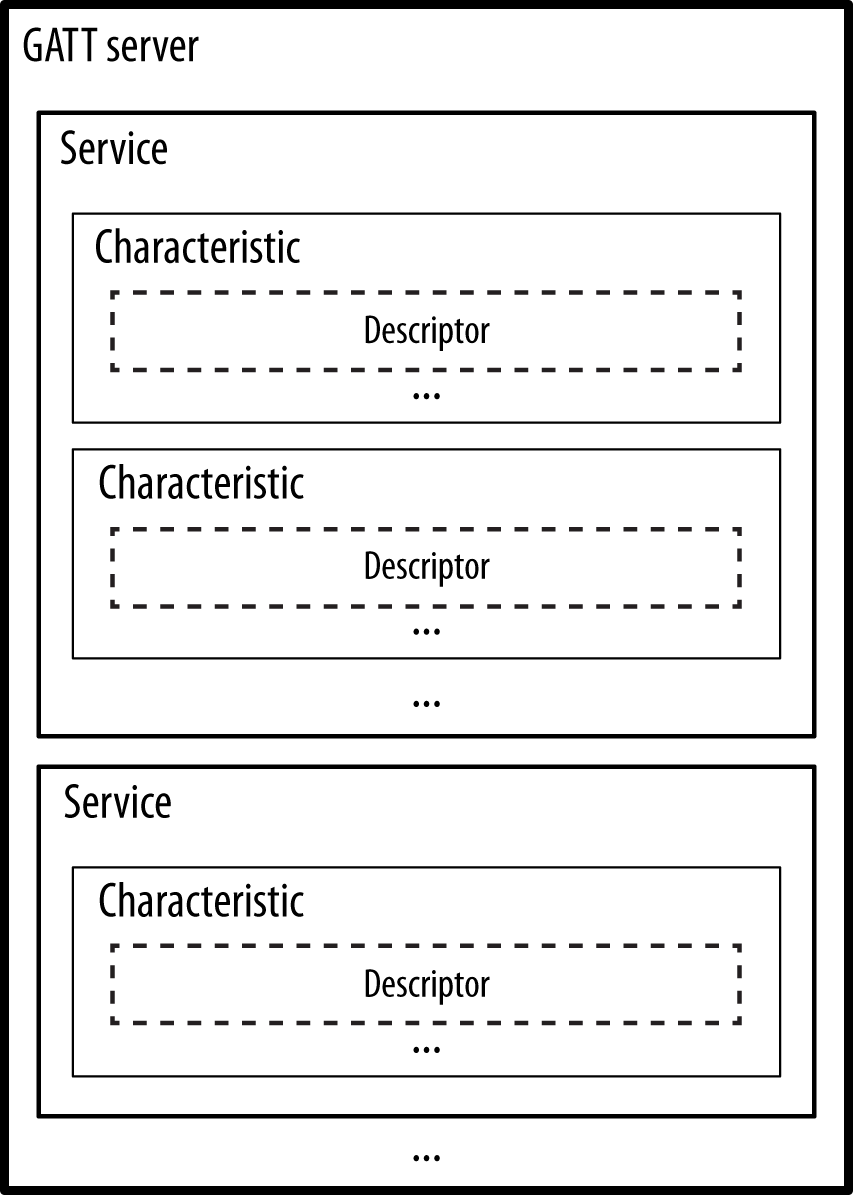
\includegraphics[scale=0.2]{images/gatt_server.png}
	\caption{GATT server}
\end{figure}
\subparagraph{Attributes in GATT}
An attribute can be seen as the basic unit of data in a GATT server. An attribute contains the following fields of data:
\begin{enumerate}
	\item \textbf{Handle} (2 bytes)
	\item \textbf{UUID} (16, 4, 2 bytes)
	\item \textbf{Permissions} (R, W, RW, None)
	\item \textbf{Value} (up to 512 bytes)
\end{enumerate}
\subparagraph{GATT operations}
\begin{itemize}
	\item \textbf{Exchange MTU} (Agreeing upon the maximum unit of transmission)
	\item \textbf{Discovery} (client finding the services at the server)
		\begin{enumerate}
			\item Service Discovery
			\item Characteristic Discovery
		\end{enumerate}
	\item \textbf{Reading Characteristics and Descriptors} (client collects information about the characteristics of various services)
	\item \textbf{Writing Characteristics and Descriptors} (client accesses and then attempts to change value of the characteristic values). The following two things are to be considered here are:
		\begin{enumerate}
			\item Insufficient Authentication (Key not available OR key send with Just Works)
			\item Insufficient Encryption (LTK available but link is not encrypted with it)
		\end{enumerate}
	\item \textbf{Server Initiated Updates} (Send asynchronously by the server whenever the value of any characteristic has been updated)
		\begin{enumerate}
			\item Characteristic Value Notification
			\item Characteristic Value Indication
		\end{enumerate}
\end{itemize}

\section{Assumptions and Dependencies}
In order for this project i.e. device driver for BlueNRG to work, the following dependencies are assumed:
\begin{itemize}
	\item A SoC system running on \textbf{Linux}.
	\item A SoC system having \textbf{SPI} support.
	\item \textbf{Bluez} on the system for testing and command line interaction.
	\item \textbf{BlueNRG} to be connected and used with the system via SPI.
\end{itemize}
The above mentioned dependencies are discussed in depth in the coming sections and chapters.
\subsection{Bluez The official Linux Bluetooth stack}
\textbf{BlueZ} is the official Linux Bluetooth protocol stack. It is an Open Source project distributed under the GNU General Public License (GPL). BlueZ kernel is part of the official Linux kernel since version 2.4.6.
\begin{figure}[ht]
	\centering
	
\includegraphics[width=3.5in, height=3in]{images/bluez_intro.png}
	\caption{Bluez the official Bluetooth stack of Linux}
\end{figure}
\subsubsection{History}
The Bluetooth technology was announced in May 1998 with the goal to create an easy usable cable replacement. But Bluetooth has proven to be more than a simple cable replacement technology with an enormous scope of applications and a rich set of standard protocol suite. The first steps into supporting Bluetooth with Linux were done by Axis Communications with their OpenBT Bluetooth Stack in April 1999. Also IBM released its BlueDrekar which was only available as binary modules. The problem of both stacks was that they are character driven, but the Bluetooth technology is for connecting devices. So it is better to integrate it into the Linux network layer and to use the socket interface as primary API.\\
On May 3, 2001, the Bluetooth protocol stack called BlueZ which was written by Qualcomm was released under GPL. The new stack followed the socket based approach. A socket in network programming represents the endpoint of a communication link. The idea is that from a software application's point of view, all data being passed through the link must go into or come out of the socket. Later it was picked up by Linus Torvalds and integrated into the Linux 2.4.6-pre2 kernel. This led to the Open Source community to support BlueZ as official Bluetooth Protocol Stack for Linux.
\subsubsection{The Bluetooth Stack}
The Bluetooth Stack is divided into three components.
\begin{enumerate}
	\item The controller
	\item The Host
	\item The Application
\end{enumerate}
Another important component is the Host Controller Interface.
\begin{figure}[ht]
	\centering
	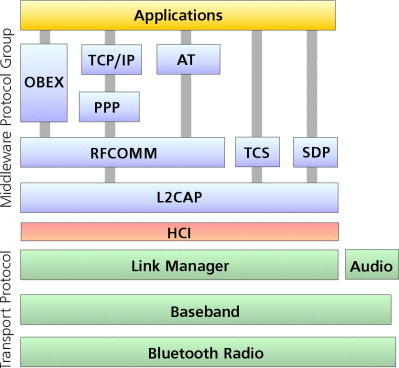
\includegraphics[scale=0.5]{images/bluetooth_stack.png}
	\caption{The Bluez Stack}
\end{figure}
The whole Bluetooth Stack has been divided into two component stacks in Linux. One portion of the stack is made part of the kernel space. The other portion is available as a separate toolkit for the users in the user-space.
\begin{figure}[ht]
	\centering
	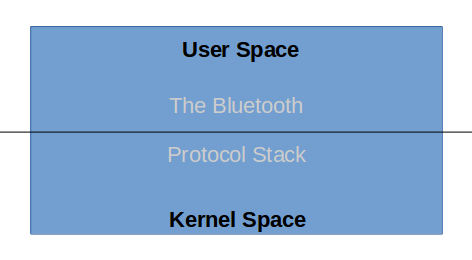
\includegraphics[width=3.5in, height=3in]{images/kernel_userspace.png}
	\caption{Stack division}
\end{figure}
The source for all of the kernel side code can be located in the Linux kernel at: \textbf{/net/Bluetooth}.\\
The Kernel side of the stack contains:
\begin{itemize}
	\item Low level protocols (L2CAP, RFCOMM, BNEP, HIDP, etc)
	\item Security (SSP, SMP)
	\item Hardware drivers
	\item Provides socket based interfaces to user space
	\begin{itemize}
		\item For data (L2CAP, RFCOMM, SCO, HCI)
		\item For control (MGMT, HCI, BNEP, HIDP)
	\end{itemize}
\end{itemize}
The source for the user-space side of Blue can be ne obtained from \textbf{http://www.bluez.org/download/}. It consists of the following things:
\begin{itemize}
	\item Bluetoothd
	\begin{itemize}
		\item Central daemon
		\item D-Bus interfaces for UI and other subsystems
		\item Reduces exposure to low details
		\item Extendible with plugins (eg neard for NFC)
	\end{itemize}
	\item Obexd
	\begin{itemize}
		\item Daemon for OBEX profiles
		\item D-Bus interface for UI
		\item Similar architecture to bluetoothd
	\end{itemize}
	\item Tools
	\begin{itemize}	
		\item Bluetoothctl – command line agent
		\item Btmon -HCI tracer
		\item Set of command line tools useful for testing, development and tracing
	\end{itemize}
\end{itemize}
The whole Bluez architecture is summed up by the following figure:
\begin{figure}[ht]
	\centering
	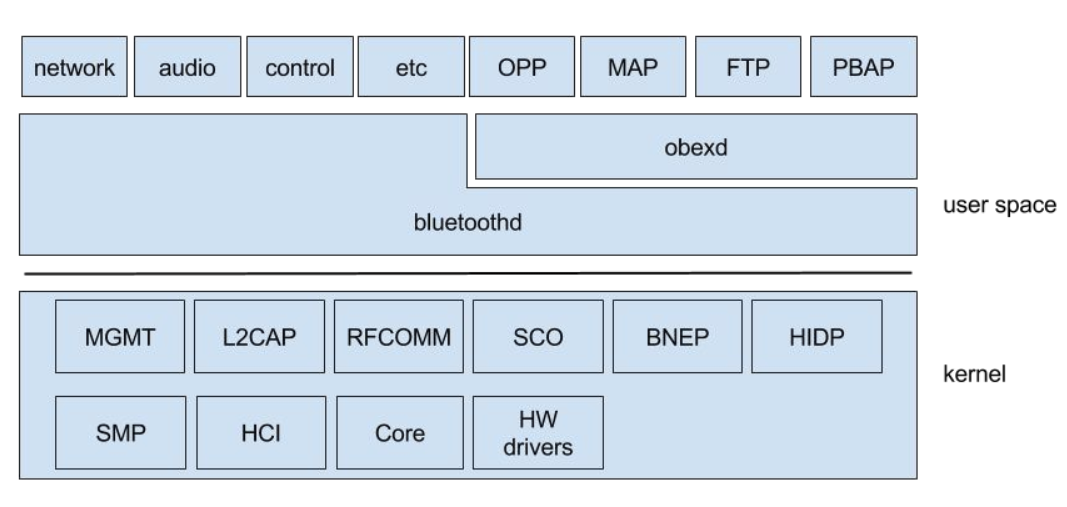
\includegraphics[width=3.5in, height=3in]{images/whole_bluez.png}
	\caption{The whole Bluez Stack}
\end{figure}

\subsection{BlueNRG}
The BlueNRG is a very low power Bluetooth Low Energy (BLE) single-mode network processor, compliant with Bluetooth specification v4.0. The BlueNRG can act as slave. The Bluetooth Low Energy stack runs on the embedded ARM Cortex-M0 core. The stack is stored on the on-chip non-volatile Flash memory and can be easily upgraded via SPI. The device comes pre-programmed with a production-ready stack image (whose version could change at any time without notice). A different or more up-to-date stack image can be downloaded from the ST web site and programmed on the device through the ST provided software tools. The BlueNRG allows applications to meet the tight advisable peak current requirements imposed by the use of standard coin cell batteries. The maximum peak current is only 10 mA at 1 dBm of output power. Ultra low-power sleep modes and very short transition times between operating modes allow very low average current consumption, resulting in longer battery life. The BlueNRG offers the option of interfacing with external microcontrollers using SPI transport layer.
\subsubsection{General Description}
The BlueNRG is a single-mode Bluetooth low energy slave network processor, compliant with the Bluetooth specification v4.0.\\
It integrates a 2.4 GHz RF transceiver and a powerful Cortex-M0 microcontroller, on which a complete power-optimized stack for Bluetooth single mode protocol runs, providing:
\begin{itemize}
	\item Slave role support
	\item GAP: peripheral, broadcaster roles
	\item ATT/GATT: client and server
	\item SM: privacy, authentication and authorization
	\item L2CAP
	\item Link Layer: AES-128 encryption and decryption
\end{itemize}
An on-chip non-volatile Flash memory allows on-field Bluetooth low energy stack upgrade.\\
The device allows applications to meet the tight advisable peak current requirements imposed by the use of standard coin cell batteries. If the high efficiency embedded DC-DC step-down converter is used, the maximum input current is only 15 mA at the highest output power (+8 dBm). Even if the DC-DC converter is not used, the maximum input current is only 29 mA at the highest output power, still preserving battery life.\\
Ultra low-power sleep modes and very short transition time between operating modes result in very low average current consumption during real operating conditions, providing very long battery life.\\
Two different external matching networks are suggested: standard mode (TX output power up to +5 dBm) and high power mode (TX output power up to +8 dBm).\\
The external host application processor, where the application resides, is interfaced with the BlueNRG through an application controller interface protocol based on a standard SPI interface.
\begin{figure}[ht]
	\centering
	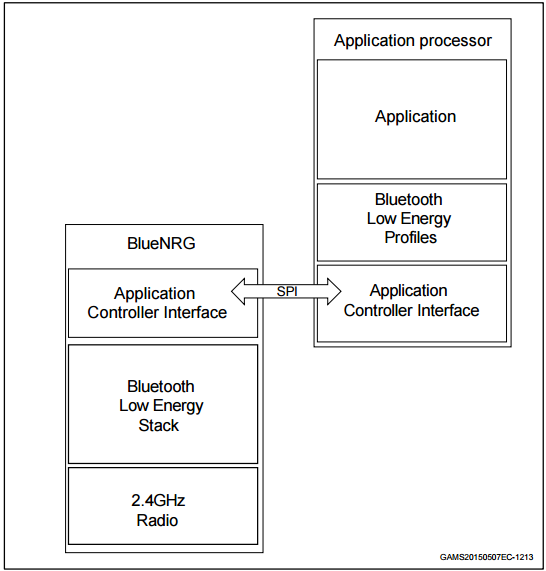
\includegraphics[width=3.5in, height=3in]{images/bluenrg_spi.png}
	\caption{BlueNRG SPI Interface}
\end{figure}
\subsubsection{Pin Description}
\begin{table}[ht]
	\centering
	\scalebox{0.5}{
	\begin{tabular}{|K{5cm} | K{5cm} | K{3cm} | K{2cm} | K{10cm}|}
		\toprule
		\rowcolor{Gray}
		\textbf{QFN32 pins} & \textbf{WLCSP pins}  & \textbf{Name} & \textbf{I/O} & \textbf{Description} \\
		\hline
		1 & E2 & SPI\_MOSI & I & SPI\_MOSI \\
		\hline
		2 & E1 & SPI\_CLK & I & SPI\_CLK \\
		\hline
		3 & D2 & SPI\_IRQ & O & SPI\_IRQ \\
		\hline
		4 & D1 & TEST1 & IO & Test pin \\
		\hline
		5 & C1 & VBAT3 & VDD & 2.0-3.6 battery voltage input \\
		\hline
		6 & C2 & TEST2 & IO & Test pin connected GND \\
		\hline
		7 & B1 & TEST3 & IO & Test pin connected GND \\
		\hline
		8 & B2 & TEST4 & IO & Test pin connected GND\\
		\hline
		9 & A1 & TEST5 & IO & Test pin connected GND\\
		\hline
		10 & B3 & TEST6 & IO & Test pin connected GND\\
		\hline
		11 & A2 & TEST7 & IO & Test pin connected GND\\
		\hline
		12 & A3 & VDD1V8 & O & 1.8 V digital core\\
		\hline
		13 & A4 & TEST8 & IO & Test pin not connected\\
		\hline
		14 & A5 & TEST9 & IO & Test pin not connected\\
		\hline
		15 & B4 & TEST11 & IO & Test pin not connected (QFN32), Test pin connected to GND (WLCSP)\\ 
		\hline
		16 & B5 & TEST12 & IO & Test pin not connected (QFN32), Test pin connected to GND (WLCSP) \\
		\hline
		17 & A6 & FXTAL1 & I & 16/32 MHz crystal\\
		\hline
		18 & B6 & FCTAL0 & I & 16/32 MHz crystal\\
	\bottomrule
	\end{tabular}}
	\caption{BlueNRG Pin Description part-I}
\end{table}
\begin{table}[ht]
	\centering
	\scalebox{0.5}{
	\begin{tabular}{|K{5cm} | K{5cm} | K{3cm} | K{2cm} | K{10cm}|}
		\toprule
		\rowcolor{Gray}
		\textbf{QFN32 pins} & \textbf{WLCSP pins}  & \textbf{Name} & \textbf{I/O} & \textbf{Description} \\
		19 & - & VBAT2 & VDD & 2.0-3.6 nattery voltage input\\
		\hline
		20 & C6 & RF1 & IO & Antenna + matching circuit\\
		\hline
		21 & D6 & RF0 & IO & Antenna + matching circuit\\
		\hline
		22 & E6 & SXTAL1 & I & 32 KHz crystal\\
		\hline
		23 & E5 & SXTAL0 & I & 32 KHz crystal\\
		\hline
		24 & D5 & VBAT1 & VDD & 2.0-3.6 battery voltage input\\
		\hline
		25 & E4 & RESETN & I & Reset\\
		\hline
		26 & F6 & SMPSFILT1 & O &  SMPS output\\
		\hline
		27 & - & NO\_SMPS & I & Power management strategy selection\\
		\hline
		28 & F5 & SMPSFILT2 & IO & SMPS input-ouput\\
		\hline
		29 & F3 & VDD1V2 & O & 1.2 V digital core\\
		\hline
		30 & E3 & TEST10 & IO & TEST pin connected to GND\\
		\hline
		31 & F2 & SPI\_CS & I & SPI\_CS\\
		\hline
		32 & F1 & SPI\_MISO & O & SPI\_MISO\\
		\hline
		- & C3 & GND & GND & Ground\\
		\hline
		- & D3 & GND & GND & Ground\\
		\hline
		- & D4 & GND & GND & Ground\\
		\hline
		- & F4 & SMPS-GND & GND & SMPS ground\\
	\bottomrule
	\end{tabular}}
	\caption{BlueNRG Pin Description part-II}
\end{table}
\subsubsection{Core, Memory and Peripherals}
The device contains an ARM Cortex-M0 microcontroller core that supports ultra-low leakage state retention mode and almost instantaneously returning to fully active mode on critical events. \\
The memory subsystem consists of 64 KB Flash, and 12 KB RAM , divided in two blocks of 6 KB (RAM1 and RAM2). Flash is used for the M0 program. No RAM or FLASH resources are available to the external microcontroller driving the BlueNRG.\\
The application controller interface (ACI) uses a standard SPI slave interface as transport layer, basing in five physical wires:
\begin{itemize}
	\item 2 control wires (clock and slave select) 
	\item 2 data wires with serial shift-out (MOSI and MISO) in full duplex 
	\item 1 wire to indicate data availability from the slave
\end{itemize}
\begin{table}[ht]
	\centering
	\scalebox{0.8}{
		\begin{tabular}{|c|c|c|c|}
			\toprule
			\rowcolor{Gray}
			\textbf{Name} & \textbf{Direction} &\textbf{Width} &\textbf{Description} \\
			\hline
			SPI\_CS & In & 1 & SPI slave select = SPI enable\\
			\hline
			SPI\_CCL & In & 1 & SPI clock (max 8MHz)\\
			\hline
			SPI\_MOSI & In & 1 & Master output, slave input\\
			\hline
			SPI\_MISO & Out & 1 & Master input, slave output\\
			\hline
			SPI\_IRQ & Out & 1 & Slave has data for master\\
			\bottomrule
		\end{tabular}
	}
	\caption{SPI Description}
\end{table}
All the SPI pins have an internal pull-down except for the CSN that has a pull-up. All the SPI pins, except the CSN, are in high impedance state during the low-power states. The IRQ pin needs a pull-down external resistor.
\subsubsection{Power Management}
The device integrates both a low dropout voltage regulator (LDO) and a step-down DC-DC converter, and one of them can be used to power the internal circuitry. However even when the LDO is used, the stringent maximum current requirements, which are advisable when coin cell batteries are used, can be met and further improvements can be obtained with the DC-DC converter at the sole additional cost of an inductor and a capacitor.
\subsubsection{Bluetooth Low Energy Radio}
The device integrates an RF transceiver compliant with the Bluetooth specification and the standard national regulations in the unlicensed 2.4 GHz ISM band. The RF transceiver requires very few external discrete components. It provides 96 dB link budgets with excellent link reliability, keeping the maximum peak current below 15 mA. In Transmit mode, the power amplifier (PA) drives the signal generated by the frequency synthesizer out to the antenna terminal through a very simple external network. The power delivered as well as the harmonic content depends on the external impedance seen by the PA.
\subsubsection{Operating Modes}
Several operating modes are defined for the BlueNRG:
\begin{itemize}
	\item Reset mode
	\item Sleep mode 
	\item Standby mode 
	\item Active mode 
	\item Radio mode 
	\begin{itemize}
		\item Receive Radio mode 
		\item Transmit Radio mode
	\end{itemize}
\end{itemize}
In Reset mode, the device is in ultra-low power consumption: all voltage regulators, clocks and the RF interface are not powered. The device enters Reset mode by asserting the external reset signal. As soon as it is de-asserted, the device follows the normal activation sequence to transit to Active mode. \\
In Sleep mode either the low speed crystal oscillator or the low speed ring oscillator are running, whereas the high speed oscillators are powered down as well as the RF interface. The state of the device is retained and the content of the RAM is preserved. Depending on the application, part of the RAM (RAM2 block) can be switched off during sleep to save more power (refer to stack mode 1, described in UM1868). \\
While in Sleep mode, the device waits until an internal timer expires and then it goes into Active mode. The transition from Sleep mode to Active mode can also be activated through the SPI interface. \\
Standby mode and Sleep mode are equivalent but the low speed frequency oscillators are powered down. In Standby mode the device can be activated through the SPI interface. \\
In Active mode the device is fully operational: all interfaces, including SPI and RF, are active as well as all internal power supplies together with the high speed frequency oscillator. The MCU core is also running. \\
Radio mode differs from Active mode as also the RF transceiver is active and it is capable of either transmitting or receiving.
\begin{figure}[ht]
	\centering
	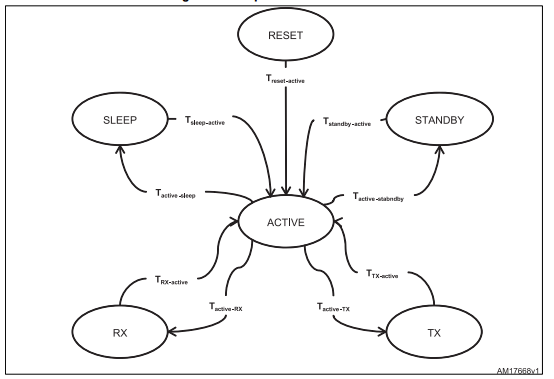
\includegraphics[width=3.5in, height=3in]{images/operating_modes.png}
	\caption{BlueNRG Operating Modes}
\end{figure}
\begin{table}[ht]
	\centering
	\scalebox{0.7}{
		\begin{tabular}{|K{2cm}| K{4cm} | K{2cm}|K{2cm}|K{2cm}|K{2cm}|K{2cm}|K{2cm}|K{2cm}|}
			\toprule
			\rowcolor{Gray}
			\textbf{State} & \textbf{Digital LDO} & \textbf{SPI} & \textbf{LSOSC} & \textbf{HSOSC} & \textbf{Core} & \textbf{RF synt.} & \textbf{RX chain} & \textbf{TX chain} \\
			\hline
			Reset & OFF Register contents lost & OFF & OFF & OFF & OFF & OFF & OFF & OFF \\
			\hline
			Standby & ON Register contents retained & ON & OFF & OFF & OFF & OFF & OFF & OFF \\
			\hline
			Sleep & ON Register contents retained & ON & ON & OFF & OFF & OFF & OFF & OFF \\
			\hline
			Active & ON Register contents retained & ON & . & ON & ON & OFF & OFF & OFF \\
			\hline
			RX & ON Register contents retained & ON & . & ON & ON & ON & ON & OFF \\
			\hline
			TX & ON Register contents retained & ON & . & ON & ON & ON & OFF & ON\\
			\bottomrule
		\end{tabular}
	}
	\caption{BlueNRG operating modes summary}
\end{table}


\section{Product Perspective}
BlueNRG is a network processor. This means it implement in it, the stack of both the host and the controller. But for the intent of this project, we are interested only in the controller stack of BlueNRG as the host part of the stack will be provided by a Linux host. As is defined in the specification a host and a controller must communicate using the HCI protocol. And Bluez is of course capable of providing this interface to our controller: BlueNRG. Since BlueNRG uses SPI as the transport layer, there is a need to write a SPI driver that can take HCI commands from Bluez stack and send them over to BlueNRG. The response to HCI commands is of course HCI events. These are communicated using the same channels i.e. SPI. \\
Once this host and controller setup is ready, it is time to communicate with another Bluetooth Low Energy complaint device. The communication between this other device and our host (the Linux machine) will happen through one of many Bluetooth Low Energy profiles in the application layer. The driver and BlueNRG need not concern itself with what these applications are. All it needs to care about is the HCI commands that is going to receive from the host over SPI and sending back appropriate responses for the send commands. This is possible because any operation that is needed to performed by the application will eventually be converted into a HCI command. All of this is taken care of by the Bluez stack between its user-space and then the kernel side components discussed earlier. \\
The follow of control or data is summarized in the following flow diagram.

\section{Flow Diagram}
\begin{figure}[ht]
	\centering
	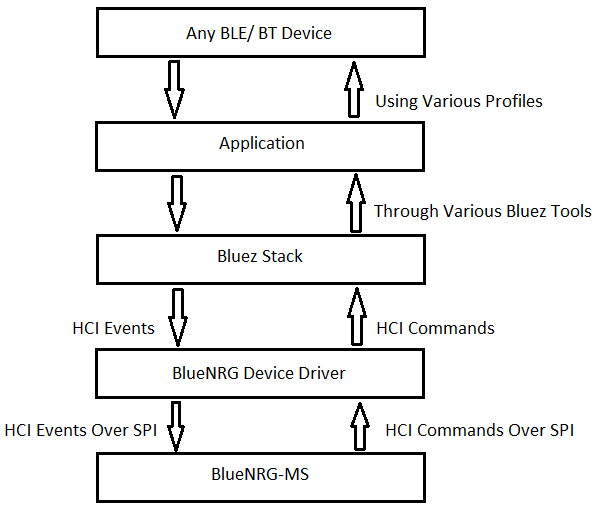
\includegraphics[scale=0.5]{images/flow_chart.png}
	\caption{Flow Chart}
\end{figure}


	\newpage

	\chapter{Development and Implementation}
\section{The Linux Kernel}
The Linux kernel is a monolithic Unix-like computer operating system kernel. The Linux operating system is based on it and deployed on both traditional computer systems such as personal computers, servers and small system on chip computers; usually in the form of Linux distributions, and on various embedded devices such as routers, wireless access points, PBXes, set-top boxes, FTA receivers, smart TVs, PVRs and NAS appliances. The Android operating system for tablet computers, smartphones and smart-watches is also based atop the Linux kernel.\\
The Linux kernel was conceived and created in 1991 by Linux Torvalds for his personal computer and with no cross-platform intentions, but has since expanded to support to huge array of computer architecture, many more than other operating systems or kernels. Linux rapidly attracted developers and users who adopted it as the kernel for other free software projects, notably the GNU Operating System. The Linux kernel has received contributions from nearly 12,000 programmers from more than 1,200 companies, including some of the largest software and hardware vendors.
\subsection{The Linux Device Driver Model}
Linux today supports more hardware devices than any other operating system in the history of the world. It does this using a development model significantly different from the familiar Windows device driver model. The Linux development process continues to evolve to better support the needs of Independent Hardware Vendors (IHVs), distributions, and other members of the community, and the advantages of the Linux model are increasing with time. While Linux will not provide a stable source or binary interface for driver developers, IHVs should familiarize themselves with a number of useful projects, many sponsored by the Linux Foundation, that ease driver development, including the Hardware NDA program, the Linux Drivers Project, and the Driver Backport Workgroup. When IHVs engage with the Linux community, they almost invariably find that the Linux driver model provides significant benefits that lower their costs while producing better drivers.
\subsubsection{Overview}
A fundamental purpose for operating systems (OSes) is to serve as an abstraction layer between applications and hardware to enable interoperability. An IHV wants their hardware to be able to make use of all the relevant features of an  OS, and an  OS  wants to take full advantage of the hardware it's running on. Since both the  OS and the hardware tend to add and to rearrange features over time, it is a dynamic interaction. What everybody wants is for the hardware to “Just Work” without hassles or support calls.\\
Today, Linux works with more devices than any other  OS  in the history of the world.
\subsubsection{Driver Model}
The Linux driver model is different. For users, the goal is to provide the “Just Works” experience. The Linux model is that IHVs get the source code for their driver accepted into the mainline kernel. This entails a public peer review process to ensure that the driver code is of sufficient quality and does not have obvious bugs or security risks. Linux has neither a stable binary driver ABI nor a stable source-code driver Application Programming Interface (API). That is, there is no guarantee that an interface provided in one version of the kernel will be available in the next version, and portions of the ABI and  API  change in every kernel release.\\
By contrast, the Linux kernel does provide a stable user-space interface for Linux applications. These applications essentially have a contract with the Linux kernel that the user-space binary interfaces they rely on will continue to work consistently over time. That's why a pre-compiled Linux application can run correctly on multiple distributions and multiple versions. The underlying implementation of the user-space binary interfaces can and does change, but even an application compiled for pre-1.0 Linux will run correctly on the latest kernel. This is the opposite of device drivers, which have no guarantee whatsoever that any interface they rely on, whether binary or source, will remain consistent between versions of the kernel.\\
Counterintuitive though it might be from a proprietary viewpoint, this lack of internal kernel interface stability is preferable because both the kernel code and all of the drivers relying on it are open source. In fact, driver code is an integral part of the Linux operating system, not a second-class add-on. Once a driver is accepted into the mainline kernel, it will be maintained over time as internal kernel interfaces change. That is, when a subsystem maintainer accepts a patch to make an incompatible change to a kernel interface, that patch will simultaneously upgrade every driver that relies on the interface. And, new drivers and any upgrades to them automatically flow downstream from the mainline kernel to all Linux distributions.\\
The key strength of this approach from the user's viewpoint is that, in happy contrast with proprietary operating systems like Windows Vista, once a device is working on a given version of Linux, that support continues through all future versions. (Devices are generally only removed when they have become so rare that no users can be found.) In Linux, hardware support only gets better; it never gets worse.\\
From the IHV's point of view, the big benefit is that an IHV's driver is maintained over time by the community, meaning that other people fix, tune, and add features to the driver. When internal kernel interfaces change in each new  OS  release, IHVs don't need to write and release a new driver; their driver is upgraded automatically. Obsolete interfaces can be deprecated and removed rather than being maintained indefinitely. Common subsystems can be factored out of drivers, enabling leaner, less buggy device drivers while adding more functionality for all hardware. This improves the stability, security, and maturity of both the OS and the driver.\\
In addition, the Linux model enables cross-architecture driver support nearly for free. Even when an IHV only tests their driver on one chip architecture, interested developers ensure that the driver works with every architecture that Linux supports, which is more than any other  OS  in history. The strength of this approach has been especially apparent over the last decade as many chip architectures have moved from the 32 to 64 bits. Nearly all Linux drivers were quickly updated to support these newer architectures, while driver support for 64-bit Windows Vista even on the highest volume x86 architecture remains extremely poor today.\\
The biggest hurdle of the Linux driver model for some IHVs is the need to open source their driver code, which a small (but thankfully dwindling) number have been reluctant to do. Also, once a driver is accepted into the mainline, it can take up to 18 months to be deployed into an enterprise distro. It has not until now been convenient to backport the driver to existing distros, but that is improving with the Driver Backport Workgroup.\\
Having hardware reliably supported by Linux means getting the driver accepted into the mainline kernel. Supporting an out-of-mainline open source driver creates significant, never-ending support costs for the IHV, as new versions constantly need to be released as the kernel  API  changes. Supporting an out-of-mainline binary driver means even bigger, never-ending support costs for the IHV, and directly contradicts the recent statement by a large number of kernel developers that binary drivers are “undesirable”.\\
The Linux driver model is different from the Windows model many IHVs are used to. But it is a consistent and compelling approach, and has been successful at supporting nearly the entire universe of computer hardware. Moreover, the vast majority of all IHVs have adapted to Linux and have thriving businesses that work with the Linux driver development model.
\subsection{Overview of SPI support in Linux}
\subsubsection{What is SPI?}
The "Serial Peripheral Interface" (SPI) is a synchronous four wire serial link used to connect microcontrollers to sensors, memory, and peripherals. It's a simple "de facto" standard, not complicated enough to acquire a standardization body.  SPI uses a master/slave configuration.\\
The three signal wires hold a clock (SCK, often on the order of 10 MHz), and parallel data lines with "Master Out, Slave In" (MOSI) or "Master In, Slave Out" (MISO) signals.  (Other names are also used.)  There are four clocking modes through which data is exchanged; mode-0 and mode-3 are most commonly used.  Each clock cycle shifts data out and data in; the clock doesn't cycle except when there is a data bit to shift.  Not all data bits are used though; not every protocol uses those full duplex capabilities.\\
SPI masters use a fourth "chip select" line to activate a given SPI slave device, so those three signal wires may be connected to several chips in parallel.  All SPI slaves support chipselects; they are usually active low signals, labeled nCSx for slave 'x' (e.g. nCS0).  Some devices have other signals, often including an interrupt to the master. \\
Unlike serial busses like USB or SMBus, even low level protocols for SPI slave functions are usually not interoperable between vendors (except for commodities like SPI memory chips).
\begin{itemize}
	\item SPI may be used for request/response style device protocols, as with touchscreen sensors and memory chips.
	\item It may also be used to stream data in either direction (half duplex), or both of them at the same time (full duplex).
	\item Some devices may use eight bit words.  Others may use different word     lengths, such as streams of 12-bit or 20-bit digital samples.
	\item Words are usually sent with their most significant bit (MSB) first, but sometimes the least significant bit (LSB) goes first instead.
	\item Sometimes SPI is used to daisy-chain devices, like shift registers.
\end{itemize}
In the same way, SPI slaves will only rarely support any kind of automatic discovery/enumeration protocol.  The tree of slave devices accessible from a given SPI master will normally be set up manually, with configuration tables.\\
SPI is only one of the names used by such four-wire protocols, and most controllers have no problem handling "MicroWire" (think of it as half-duplex SPI, for request/response protocols), SSP ("Synchronous Serial Protocol"), PSP ("Programmable Serial Protocol"), and other related protocols.\\
Some chips eliminate a signal line by combining MOSI and MISO, and limiting themselves to half-duplex at the hardware level. In fact some SPI chips have this signal mode as a strapping option.  These can be accessed using the same programming interface as SPI, but of course they won't handle full duplex transfers.  You may find such chips described as using "three wire" signaling: SCK, data, nCSx. (That data line is sometimes called MOMI or SISO.) \\
Microcontrollers often support both master and slave sides of the SPI protocol.  This document (and Linux) currently only supports the master side of SPI interactions.
\subsubsection{Who uses SPI?}
Linux developers using SPI are probably writing device drivers for embedded systems boards.  SPI is used to control external chips, and it is also a protocol supported by every MMC or SD memory card.  (The older "DataFlash" cards, predating MMC cards but using the same connectors and card shape, support only SPI.)  Some PC hardware uses SPI flash for BIOS code. \\
SPI slave chips range from digital/analog converters used for analog sensors and codecs, to memory, to peripherals like USB controllers or Ethernet adapters; and more. \\
Most systems using SPI will integrate a few devices on a mainboard. Some provide SPI links on expansion connectors; in cases where no dedicated SPI controller exists, GPIO pins can be used to create a low speed "bitbanging" adapter.  Very few systems will "hotplug" an SPI controller; the reasons to use SPI focus on low cost and simple operation, and if dynamic reconfiguration is important, USB will often be a more appropriate low-pincount peripheral bus. \\
Many microcontrollers that can run Linux integrate one or more I/O interfaces with SPI modes. Given SPI support, they could use MMC or SD cards without needing a special purpose MMC, SD or SDIO controller.
\subsubsection{The SPI programming interface}
The linux/spi/spi.h header file includes kerneldoc, as does the main source code, and you should certainly read that chapter of the kernel API document.  This is just an overview, so you get the big picture before those details. \\
SPI requests always go into I/O queues.  Requests for a given SPI device are always executed in FIFO order, and complete asynchronously through completion callbacks.  There are also some simple synchronous wrappers for those calls, including ones for common transaction types like writing a command and then reading its response. \\
There are two types of SPI driver, here called: \\
Controller drivers ... controllers may be built into System-On-Chip 	processors, and often support both Master and Slave roles. 	These drivers touch hardware registers and may use DMA. 	Or they can be PIO bitbangers, needing just GPIO pins.\\ 
Protocol drivers ... these pass messages through the controller 	driver to communicate with a Slave or Master device on the 	other side of an SPI link. \\
So for example one protocol driver might talk to the MTD layer to export data to filesystems stored on SPI flash like DataFlash; and others might control audio interfaces, present touchscreen sensors as input interfaces, or monitor temperature and voltage levels during industrial processing. And those might all be sharing the same controller driver.\\
A "struct spi\_device" encapsulates the master-side interface between those two types of driver.  At this writing, Linux has no slave side programming interface. \\
There is a minimal core of SPI programming interfaces, focussing on using the driver model to connect controller and protocol drivers using device tables provided by board specific initialization code.  SPI shows up in sysfs in several locations: 
\begin{itemize}
	\item /sys/devices/.../CTLR ... physical node for a given SPI controller 
	\item /sys/devices/.../CTLR/spiB.C... spi\_device on bus "B", chipselect C, accessed through CTLR. 
	\item /sys/bus/spi/devices/spiB.C ... symlink to that physical .../CTLR/spiB.C device 
	\item /sys/devices/.../CTLR/spiB.C/modalias ... identifies the driver that should be used with this device (for hotplug/coldplug) 
	\item /sys/bus/spi/drivers/D ... driver for one or more spi*.* devices 
	\item /sys/class/spi\_master/spiB ... symlink (or actual device node) to a logical node which could hold class related state for the controller managing bus "B". All spiB.* devices share one physical SPI bus segment, with SCLK, MOSI, and MISO. 
\end{itemize}
Note that the actual location of the controller's class state depends on whether you enabled CONFIG\_SYSFS\_DEPRECATED or not.  At this time, the only class-specific state is the bus number ("B" in "spiB"), so those /sys/class entries are only useful to quickly identify busses.

\section{The C Programming Language}
C is the language of the Linux kernel. Almost all of the kernel and related applications are written in C. C is of course the language of development in this project.\\
C is a general-purpose programming language with features economy of expression, modern flow control and data structures, and a rich set of operators. C is not a ``very high level'' language, nor a ``big''one, and is not specialized to any particular area of application. But its absence of restrictions and its generality make it more convenient and effective for many tasks than supposedly more powerful languages. C was originally designed for and implemented on the UNIX operating system on the DEC PDP-11, by Dennis Ritchie. The operating system, the C compiler, and essentially all UNIX applications programs (including all of the software used to prepare this book) are written in C. Production compilers also exist for several other machines, including the IBM System/370, the Honeywell 6000, and the Interdata 8/32. C is not tied to any particular hardware or system, however, and it is easy to write programs that will run without change on any machine that supports C.\\
The C language has a very simple structure and hence is much easily converted into machine code without any overhead that may be faced when using other languages. That is why almost all of the kernel development and device drivers are done in C language only even after the introduction of so many other versatile languages like C++.

\section{Development Boards}
In order to develop and test the driver code as well as to interface the BlueNRG chip to the host via SPI, there was need for a system-on-board computer. The host of course needed to run on a Linux kernel, so the following two were the obvious choices
\subsection{Raspberry Pi}
Several generations of Raspberry Pis have been released. The first generation (Raspberry Pi 1 Model B) was released in February 2012. It was followed by a simpler and inexpensive model Model A. In 2014 the foundation released a board with an improved design in Raspberry Pi 1 Model B+. The model laid the current "mainline" form-factor. Improved A+ and B+ models were released a year later. A cut down "compute" model was released in April 2014, and a Raspberry Pi Zero with smaller size and limited input/output (I/O) and general-purpose input/output (GPIO) abilities was released in November 2015 for US\$5. The Raspberry Pi 2 which added more RAM was released in February 2015. Raspberry Pi 3 Model B released in February 2016 is bundled with on-board WiFi and Bluetooth. As of 2016, Raspberry Pi 3 Model B is the newest mainline Raspberry Pi. These boards are priced between US \$20–35.\\
All models feature a Broadcom system on a chip (SoC), which includes an ARM compatible central processing unit (CPU) and an on chip graphics processing unit (GPU, a VideoCore IV). CPU speed ranges from 700 MHz to 1.2 GHz for the Pi 3 and on board memory range from 256 MB to 1 GB RAM. Secure Digital (SD) cards are used to store the operating system and program memory in either the SDHC or MicroSDHC sizes. Most boards have between one and four USB slots, HDMI and composite video output, and a 3.5 mm phone jack for audio. Lower level output is provided by a number of GPIO pins which support common protocols like I²C. The B-models have an 8P8C Ethernet port and the Pi 3 has on board Wi-Fi 802.11n and Bluetooth.\\
The Foundation provides Raspbian, a Debian-based Linux distribution for download, as well as third party Ubuntu, Windows 10 IOT Core, RISC OS, and specialised media center distributions. It promotes Python and Scratch as the main programming language, with support for many other languages. The default firmware is closed source, while an unofficial open source is available.
The Raspberry Pi 3 model was used for preliminary development of this driver.
\begin{figure}[H]
	\centering
	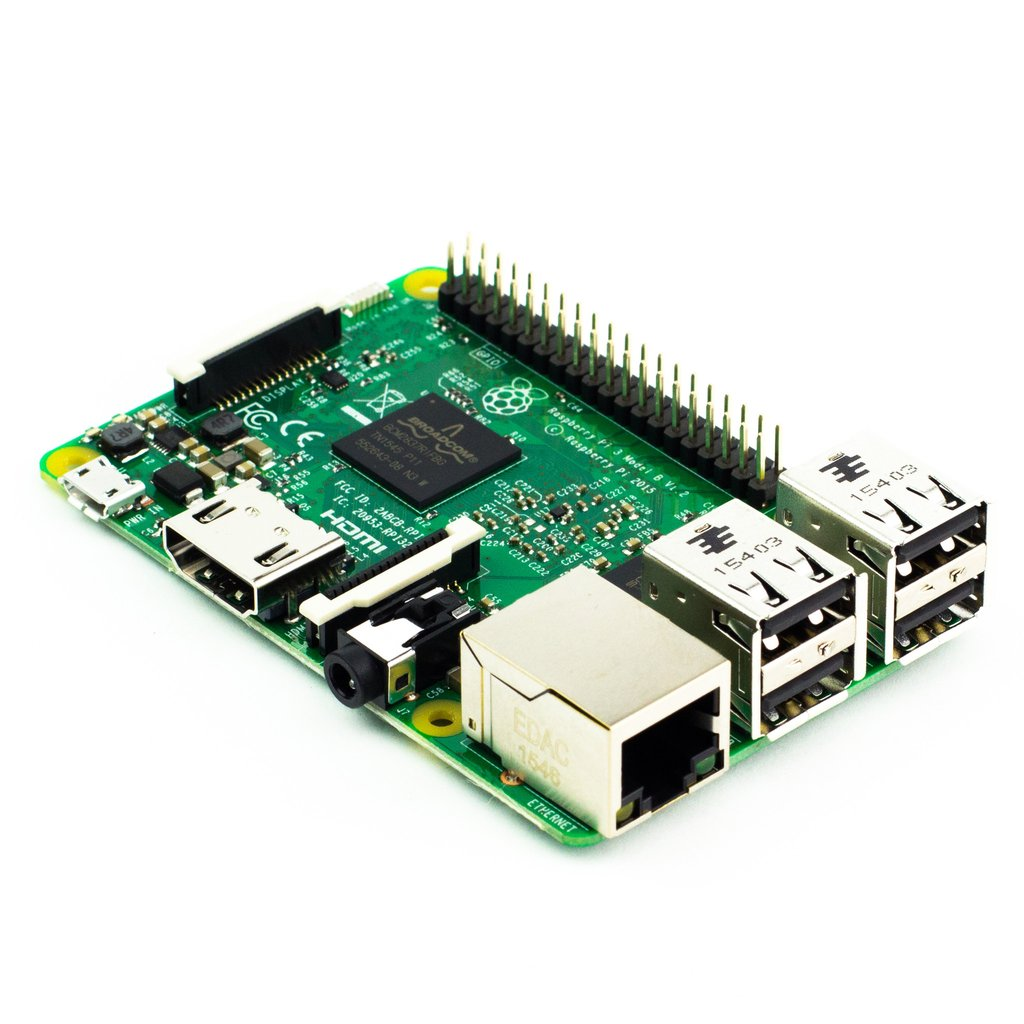
\includegraphics[width=3.5in, height=3in]{images/raspberry_pi.png}
	\caption{Raspberry Pi 3}
\end{figure}

\subsection{BeagleBone Black}
The BeagleBoard is a low-power open-source hardware single-board computer produced by Texas Instruments in association with Digi-Key and Newark element14. The BeagleBoard was also designed with open source software development in mind, and as a way of demonstrating the Texas Instrument's OMAP3530 system-on-a-chip. The board was developed by a small team of engineers as an educational board that could be used in colleges around the world to teach open source hardware and software capabilities. It is also sold to the public under the Creative Commons share-alike license. The board was designed using Cadence OrCAD for schematics and Cadence Allegro for PCB manufacturing; no simulation software was used.\\
The BeagleBone Black is the newest member of the BeagleBoard family. It is a lower-cost, high-expansion focused BeagleBoard using a low cost Sitara XAM3359AZCZ100 Cortex A8 ARM processor from Texas Instruments. It is similar to the Beaglebone,but with some features removed and some features added. The table below gives the high points on the differences between the BeagleBone and BeagleBone Black.
\begin{figure}[ht]
	\centering
	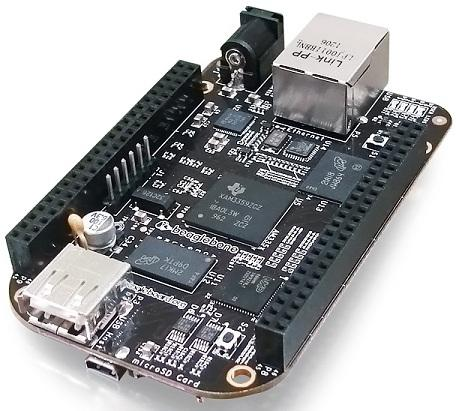
\includegraphics[width=3.5in, height=3in]{images/beaglebone_black.png}
	\caption{BeagleBone Black}
\end{figure}


\section{Tools used}
\subsection{Buildroot}
Buildroot is a set of Makefiles and patches that simplifies and automates the process of building a complete and bootable Linux environment for an embedded system, while using cross-compilation to allow building for multiple target platforms on a single Linux-based development system. Buildroot can automatically build the required cross-compilation toolchain, create a root file system, compile a Linux kernel image, and generate a boot loader for the targeted embedded system, or it can perform any independent combination of these steps. For example, an already installed cross-compilation toolchain can be used independently, while Buildroot only creates the root file system. \\
Buildroot is primarily intended to be used with small or embedded systems based on various computer architectures and instruction set architectures (ISAs), including x86, ARM, MIPS and PowerPC. Numerous architectures and their variants are supported; Buildroot also comes with default configurations for several off-the-shelf available embedded boards, such as Cubieboard, Raspberry Pi and SheevaPlug. Several third-party projects and products use Buildroot as the basis for their build systems, including the OpenWrt project that creates an embedded operating system, and firmware for the customer-premises equipment (CPE) used by the Google Fiber broadband service.\\
Multiple C standard libraries are supported as part of the toolchain, including the GNU C Library, uClibc and musl, as well as the C standard libraries that belong to various preconfigured development environments, such as those provided by Linaro. Buildroot's build configuration system internally uses Kconfig, which provides features such as a menu-driven interface, handling of dependencies, and contextual help; Kconfig is also used by the Linux kernel for its source-level configuration. Buildroot is organized around numerous automatically downloaded packages, which contain the source code of various userspace applications, system utilities, and libraries. Root file system images, which are the final results, may be built using various file systems, including cramfs, JFFS2, romfs, SquashFS and UBIFS.\\
Buildroot is free and open-source software, maintained by Peter Korsgaard and licensed under version 2 or later of the GNU General Public License (GPL). The project started in 2001, with initial intentions to serve as a testbed for uClibc. New releases are made available every three months.
\begin{figure}[ht]
	\centering
	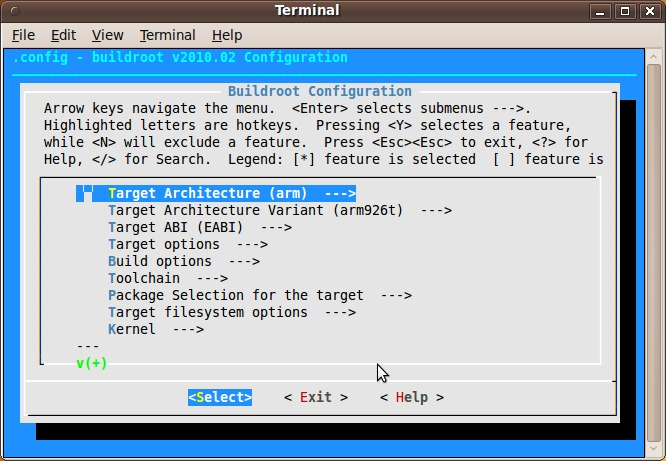
\includegraphics[width=3.5in, height=3in]{images/buildroot.png}
	\caption{Buildroot}
\end{figure}
\subsection{Cscope}
While hacking around the Linux source code it becomes very difficult to keep track of the program flow or the variable structures in your head. There isn’t any IDE to help out in source code browsing either. In such situation a tool is necessary that browses source code and is based on the terminal. This is where cscope comes into picture.\\
cscope is a programming tool which works in console mode, text-based interface, that allows computer programmers or software developers to search source code of the programming language C, with some support for C++ and Java. It is often used on very large projects to find source code, functions, declarations, definitions and regular expressions given a text string. cscope is free and released under a BSD license. The original developer of cscope is \textbf{Joe Steffen}.\\
The history of the tool goes back to the days of the PDP-11, but it is still used by developers who are accustomed to using the vi or Vim editor or other text-based editors, instead of editors based on graphical user interfaces (GUI)s. The functions in cscope are available to varying degrees in modern graphical source editors.
cscope is used in two phases. First a developer builds the cscope database. The developer can often use find or other Unix tools to get the list of filenames needed to index into a file called cscope.files. The developer then builds a database using the command cscope -b -q -k. The k flag is intended to build a database for an operating system or C library source code. It will not look in /usr/include. Second, the developer can now search those files using the command cscope -d. Often an index must be rebuilt whenever changes are made to files.\\
In software development it is often very useful to be able to find the callers of a function because this is the way to understand how code works and what other parts of the program expect from a function. cscope can find the callers and callees of functions, but it is not a compiler and it does that by searching the text for keywords. This has the disadvantages that macros and duplicate symbol names can generate an unclear graph. There are other programs that can extract this information by parsing the source code or looking at the generated object files.
cscope was created to search content within C files, but it can also be used (with some limits) for C++ and Java files.
\begin{figure}[ht]
	\centering
	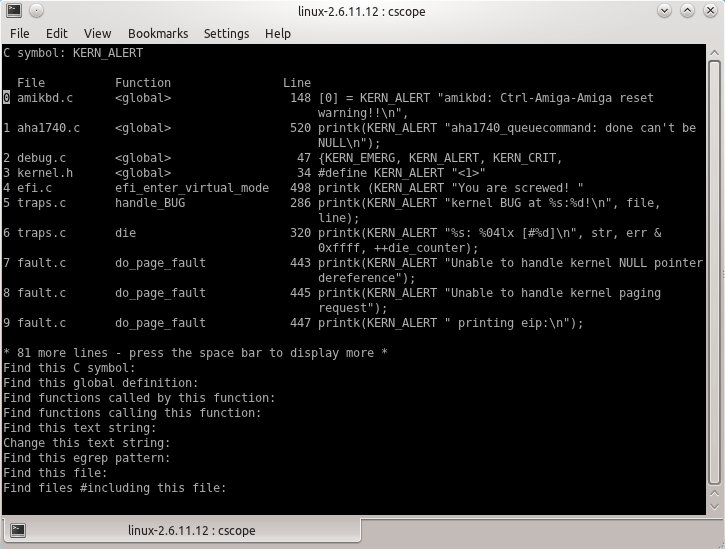
\includegraphics[scale=0.5]{images/cscope.png}
	\caption{Source Browsing through Cscope}
\end{figure}

\section{Testing}
The driver's job is to send commands from the Bluez stack to the device and get back its response. If all of this happens successfully then that should mean that the BlueNRG is able to communicate with another device using some BLE use cases.\\
Some of the use cases that can be used to test this are:
\subsection{Checking to see if BLE gets enabled} 
	\begin{enumerate}
		\item This can be done using the following command\\
			\textbf{sudo hciconfig hci0 lestates}
		\item This command should return the following output:
			\begin{figure}[ht]
			\centering
			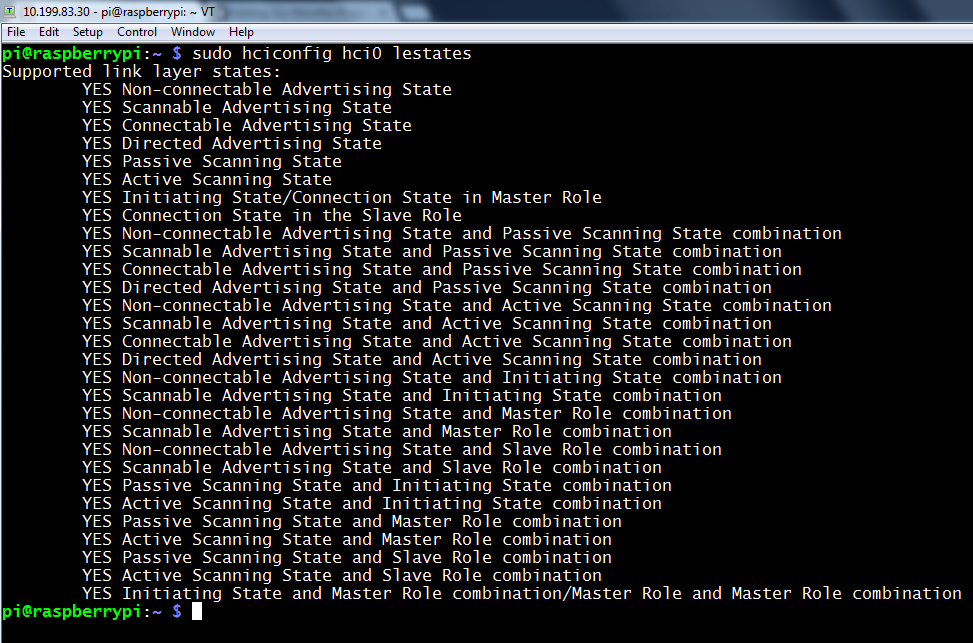
\includegraphics[scale=0.5]{images/lestates.png}
			\caption{List of LE states supported by adapter}
		\end{figure}
	\end{enumerate}
\subsection{BLE gatttool interaction} 
gatttool is one of the best methods to interact with another BLE device interactively from a Linux host. It opens an interactive session.
	\begin{enumerate}
		\item Find out the MAC\_ADDR of the other device using\\
			\textbf{sudo hcitool lescan}
			\begin{figure}[ht]
				\centering
				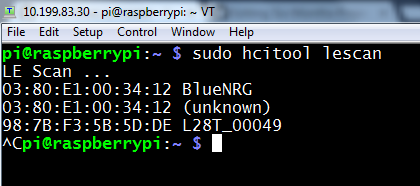
\includegraphics[scale=0.5]{images/lescan.png}
				\caption{List of LE devices scanned}
			\end{figure}
		\item Open interactive session using gatttool:\\
			\textbf{sudo gatttool -i hci0 -b MAC\_ADDR -I}
		\item In the interactive sesssion type in the following commands:\\
			\textbf{connect}
		\item Read profiles:\\
			\textbf{primary}
		\item Read all available characterstics:\\
			\textbf{char-desc}
			\begin{figure}[ht]
				\centering
				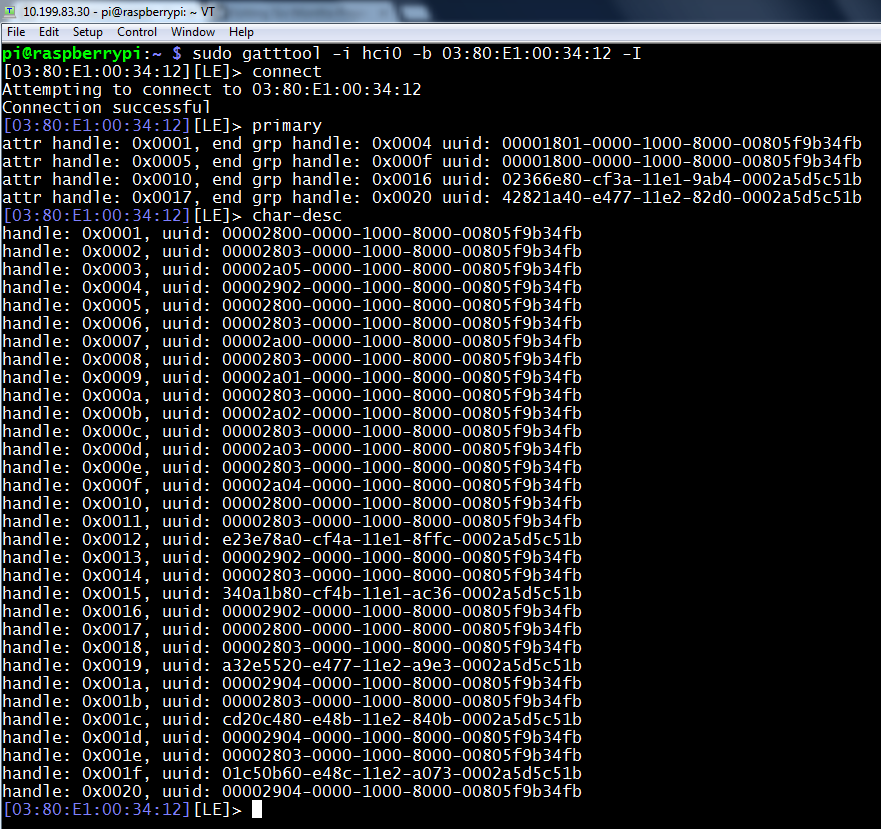
\includegraphics[scale=0.5]{images/gatttool1.png}
				\caption{GATTtool interaction part-I}
			\end{figure}
		\item Read the value of a characterstic:\\
       			\textbf{char-read-hnd The\_characterstic\_handle}
   			\item Write to a particular characterstc:\\
       			\textbf{char-write-cmd handle Value\_in\_Hex}
				\begin{figure}[ht]
				\centering
				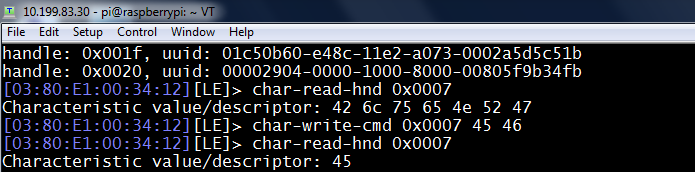
\includegraphics[scale=0.5]{images/gatttool2.png}
				\caption{GATTtool interaction part-II}
			\end{figure}
   			\item Disconnect:\\
       			\textbf{disconnect}
   			\item Quit:\\
       			\textbf{quit}
	\end{enumerate}
\subsection{Reading Beacons using BLE}
	\begin{enumerate}
		\item There is a python script that can be used for this purpose, install it:\\
			\textbf{git clone https://github.com/switchdoclabs/BeaconAirPython.git}
		\item In order to use, the following package must be installed:
			\textbf{sudo apt-get install python-bluez}
		\item Scan and Read the beacons:\\
			\textbf{cd BeanconAirPython/ble}\\
			\textbf{sudo python testblescan.py}
		\item This should list out the nearby beacons:
			\begin{figure}[ht]
				\centering
				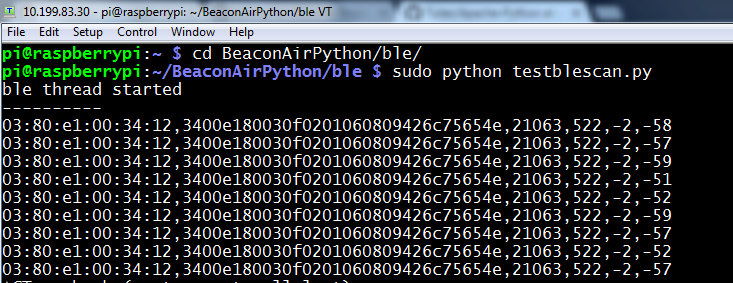
\includegraphics[scale=0.5]{images/beacon_read.png}
				\caption{Reading beacons}
			\end{figure}
	\end{enumerate}
\subsection{Advertising with Beacons}
	\begin{enumerate}
		\item Start advertising in non-connectable state:\\
			\textbf{sudo hciconfig hci0 leadv 3}\\
			\textbf{sudo hciconfig hci0 noscan}
		\item Broadcast a beacon:\\
			\textbf{sudo hcitool -i hci0 cmd 0x08 0x0008 1E 02 01 1A 1A FF 4C 00 02 15 63 6F 3F 8F 64 91 4B EE 95 F7 D8 CC 64 A8 63 B5 00 00 00 00 C8}
		\item You should see the following as output:
			\begin{figure}[ht]
				\centering
				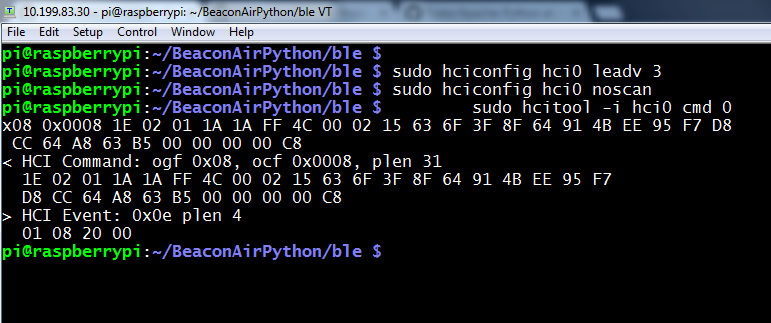
\includegraphics[scale=0.5]{images/advertising_beacons.png}
				\caption{Advertising using beacons}
			\end{figure}
	\end{enumerate}


	\newpage

	\chapter{Conclusion and Future Scope}
\section{Conclusion}
I have learnt a great deal working on this project. The learning was not limited to project only but the whole experience of working as an intern in a multinational company like STMicroelectronics was immensely educational. Being an intern, one is always challenged by the fundamental difference between classroom coaching and real industrial experience. But such a challenge is exactly the purpose of six months training.\\
The whole experience of working on this project and contributing in a few others has been very rewarding as it has given great opportunities to learn new things and get a firmer grasp on already known technologies. Here is a reiteration of some of the technologies I have encountered, browsed and learnt:
\begin{itemize}
	\item Operating System: \textbf{Linux}
	\item Language: \textbf{C}
	\item Development Host: \textbf{Raspberry Pi}, \textbf{BeagleBone Black}
	\item Integrated Build Environment: \textbf{Buildroot}
\end{itemize}
So during this project I learnt all the above things. Above all I got to know how software is developed and how much work and attention to details is required in building even the most basic of components of any project. Planning, designing, developing code, working in a team, testing, etc. these are all very precious lessons in themselves. 

\section{Future Scope}
Bluetooth Low Energy is a relatively new technology. This implies that there is a long road ahead of more features, more research and more hardware for this technology. As such there is always room for inclusion in the Linux kernel for all of this. If the completely new hardware is introduced then it becomes very important to have its driver included in Linux. This is not just have the support for the device in Linux but it also acts like an endorsement for the device that its driver has been registered with the coveted Linux kernel.\\
Talking specifically about some of the other Bluetooth Low Energy solutions by ST, following two come to immediate consideration that can also be driven by a Linux host by means of device driver written in a manner much similar to BlueNRG:
\begin{enumerate}
	\item \textbf{BlueNRG-MS}
	\item \textbf{BlueNRG 1}
\end{enumerate}
The continuous need for more software related to BLE in Linux is not just restricted to device driver development. Bluez is the official Bluetooth stack for Linux but even it does not implement everything in the Bluetooth 4.1 specification. Some features are missing and are intended for the future. Also since with new specification releases, more and more features get introduced into the technology. So the stack will also have to sustain with the specification. Some of the things that are not yet implemented in Bluez but are part of the Bluetooth specification are:
\begin{itemize}
	\item Random address support
	\item Privacy
	\item GATT server API
	\item Register Application API
	\item Better connection management
	\item Characteristic descriptors
\end{itemize}
More such issues can be found in the TODO file of Bluez source code package.


	\newpage
\end{document}
